\documentclass[11pt]{article}

\usepackage{fullpage}
\usepackage[utf8]{inputenc}
\usepackage[american]{babel}
\usepackage{csquotes}
\usepackage{listings}
\usepackage[table]{xcolor}
\usepackage{amssymb}
\usepackage{amsmath}
\usepackage{fancyhdr}
\usepackage{lastpage}
\usepackage{parskip}
\usepackage{abstract}
\usepackage{url}
\usepackage{float}
\usepackage{enumitem}
\usepackage{fancybox}
\usepackage{amsmath}
\usepackage{graphicx}
\usepackage[bottom]{footmisc}
\usepackage{makecell}
\usepackage{ifthen}
\usepackage{listings}
\usepackage{parcolumns}
\usepackage{subcaption}
\usepackage{drawstack}
\usepackage{pdfpages}
\usepackage{makecell}
\usepackage{setspace}
\usepackage{algorithm}
\usepackage{algpseudocode}
\usepackage{hyperref}

\usetikzlibrary{shapes.multipart,arrows}

\usepackage[backend=biber]{biblatex}
\bibliography{report}

\setcounter{secnumdepth}{3} % only chapter and sections will be numbered
\setcounter{tocdepth}{3}    % entries down to \subsubsections in the TOC

% constants
\newcommand{\COURSE}{Bachelor Thesis}
\newcommand{\TITLE}{Abstract Machine for Modern Languages}
\newcommand{\DATE}{June 2015}
\newcommand{\thename}{Matisse}

\addto\captionsamerican{\renewcommand{\contentsname}{Table of Contents}}

%%% Local Variables:
%%% mode: latex
%%% TeX-master: "report"
%%% End:

% generalized stuff
\newcommand{\code}[1]{\texttt{#1}}
\newcommand{\term}[1]{\textit{#1}}

% colors
\definecolor{Brown}{cmyk}{0,0.81,1,0.60}
\definecolor{OliveGreen}{cmyk}{0.64,0,0.95,0.40}
\definecolor{CadetBlue}{cmyk}{0.62,0.57,0.23,0}
\definecolor{lightlightgray}{gray}{0.95}
\definecolor{lightgray}{gray}{0.85}
\definecolor{sh_comment}{rgb}{0.12, 0.38, 0.18}
\definecolor{sh_keyword}{rgb}{0.37, 0.38, 0.75}
\definecolor{sh_string}{rgb}{0.06, 0.10, 0.98}

% listings
\lstset{
  basicstyle=\small\ttfamily,
  stringstyle=\color{sh_string},
  keywordstyle = \color{sh_keyword}\bfseries,
  commentstyle=\color{sh_comment},
  backgroundcolor=\color{lightlightgray},
  frame=single,
  rulecolor=\color{lightgray},
  framesep=3pt,
  numbersep=5pt,
  xleftmargin=10pt,
  xrightmargin=10pt,
  showspaces=false,
  showstringspaces=false,
  tabsize=4,
  aboveskip=5pt,
  belowskip=5pt,
  lineskip=2pt,
  captionpos=b,
  numbers=left,
  numberstyle=\tiny,
  stepnumber=1,
  numbersep=100pt,
  breaklines,
  numbersep=5pt,
  breakatwhitespace=false,
  showspaces=false,
  showtabs=false
}

 % TODO
\lstdefinelanguage{bytecode}{
  keywords={fn, pop},
  keywordstyle=\color{blue}\bfseries,
  ndkeywords={class, export, boolean, throw, implements, import, this},
  ndkeywordstyle=\color{darkgray}\bfseries,
  identifierstyle=\color{black},
  sensitive=false,
  comment=[l]{//},
  morecomment=[s]{/*}{*/},
  commentstyle=\color{purple}\ttfamily,
  stringstyle=\color{red}\ttfamily,
  morestring=[b]',
  morestring=[b]"
}

\let\oldcite=\cite
\renewcommand\cite[1]{\ifthenelse{\equal{#1}{NEEDED}}{[citation~needed]}{\oldcite{#1}}}


\pagestyle{fancy}
\fancyhf{}
\setlength{\parindent}{0pt}
\setlength{\headheight}{15pt}
\setlength{\headsep}{25pt}
\lhead{\TITLE}
\chead{}
\rhead{\leftmark}
\cfoot{Page \thepage{} of~\pageref{LastPage}}

\begin{document}
%%% Local Variables:
%%% mode: latex
%%% TeX-master: "report"
%%% End:

\newcommand*\formatname[2]{
  \leavevmode
  \rlap{\textit{#1}}
  \hspace{0.3\linewidth}
  \code{#2}}

\begin{titlepage}

\thispagestyle{empty}

\begin{flushright}
  
\includegraphics[width=9cm]{images/dtu}
\end{flushright}

\vskip20mm
\begin{center}
  \vskip5mm
  \huge\textbf{\TITLE}
  \vskip5mm
  \Large \COURSE
  \vskip3mm
  \large \DATE
\end{center}
\vfill

\begin{flushleft}
  \normalsize
  \formatname{Markus Veie Færevaag}{s123692} \par
  \formatname{Simon Altschuler}{s123563} \par
  \vskip2cm
  
\includegraphics[width=7cm]{images/dtu-compute}
\end{flushleft}

\end{titlepage}

\clearpage

\onehalfspacing{}

\section*{Abstract}
\label{sec:abstract}
Abstract machines are used everywhere that code is to be executed, be it web
browsers, desktop applications or embedded devices. The industry standard
abstract machines available today are predominantly designed with imperative and
object-oriented languages in mind, often resulting in awkward ad-hoc
implementations for trending paradigms like functional and dynamic
languages. This thesis presents an attempt to design and implement a new
abstract machine called \thename{} whose ambition is to efficiently and
elegantly support both traditional and emerging paradigms. We describe the
instruction set supported by \thename{} and detail how the implementation was
developed. Finally we present a performance and architectural analysis which
indicates that while \thename{} is not on par with industry standards, it has
potential to fulfill its vision. The result is a working abstract machine that
is capable of executing simple programs in an elegant and flexible manner.

%%% Local Variables:
%%% mode: latex
%%% TeX-master: "../report"
%%% End:

\clearpage

\section*{Acknowledgements}
\label{sec:acknow}
We would like to express deepest our appreciation to our adviser, Associate
Professor Sven Karlsson, for your guidance and expert knowledge.

% TODO: the work sven has done on design, spec etc.

In addition, a thank you to our second adviser, PhD Student Maxwell Walter, for
your valuable insight.

%%% Local Variables:
%%% mode: latex
%%% TeX-master: "../report"
%%% End:

\clearpage

\tableofcontents
\clearpage

\section{Introduction}
\label{sec:intro}
%%% Local Variables:
%%% mode: latex
%%% TeX-master: "../report"
%%% End:

% Motivation

New programming languages are coming into existence at a very rapid pace. Tools
for creating languages are in abundance, and even the beginning student of
computer science will most likely posses the knowledge to use them. When
languages become pass\'e or fundamental shortcomings are discovered, the
prevalent solution seems to be the creation of new and improved languages
instead of updating the existing. All of this has resulted in hundreds, if not
thousands, of available languages in a myriad of styles and paradigms for just
as many different purposes.

The world of language paradigms has become something of a religious matter for
many. Some swear by the functional approach, others by object orientation and
some insist on procedural languages, the rest on something in between. Each
require distinct and often very complex implementations that are inherently
difficult to optimize and evolve as the feature sets expand. Static or dynamic
typing is another question that divides people that of like pineapple on
pizza; strong arguments exist for both and it often comes down to a matter of
taste and preference.

Intrinsic to a language is a platform on which to be executed, be it a desktop
computer, cell phone, embedded device or essentially any other digital
device. Historically, languages where developed to be used on a single platform,
often written for a particular processor architecture, but nowadays only the
most domain specific languages can make due with that. Any language that desires
widespread adaptation must work on a multitude of devices, and not only are
there scores of architectures on the market, they are also very different in
terms of execution models and what technical primitives they provide.

Altogether language and platform diversity has grown beyond what most would have
believed when the first programmable machines appeared. That is why abstract
machines are becoming increasingly relevant to modern computer science.

In brief, an abstract machine relieves language creators of the burden of
architecture specific implementation. By providing a unified platform they
abstract away the underlying hardware specifics and can provide a higher level
of expressiveness than the bare-metal counterpart.

There are many abstract machines available today, and several are industrial
strength systems that are in use on billions of devices. What they generally
lack however, is flexibility in terms of language support. Usually they are
designed with a specific language, or family or languages, in mind which
obviously comes at the cost of adaptability by other languages. Emerging
paradigms such as dynamic and functional\footnote{Functional languages have been
  around for a long time, but are becoming increasingly popular} languages are
not well suited for the currently available abstract machines.

Having written a compiler for a functional language\footnote{In the course
  ``02122 Software Technology Project F14'' at DTU Compute} we are aware of the
issues faced by compiling code to traditional platforms, and have felt the need
for something better.

\subsection{The Multi-Paradigm Abstract Machine}

In response to the issues of today's available systems, the main ambition of
this project is to provide an abstract machine that is well suited for a
multitude of programming languages of different paradigms. Our system exposes
low level primitives that are relevant for system programming while being
efficient, expressive and secure enough as a higher level programming
environment.

To facilitate the above, an instruction set has been defined that covers the
requirements of many language paradigms in a solid, compact fashion with the
support of a corresponding execution model.

The instruction set and execution model have been implemented in the abstract
machine that we have named \thename{}.

\subsection{Status of the Implementation}

The \thename{} specification is an extensive document which covers a lot of
features. We have focused on implementing a subset of the specification that
enabled us to run simple programs and perform some benchmarking tests. Thus, the
full specification as is found in Appendix~\ref{sec:appendix:spec} is not
implemented. The Design chapter (Section~\ref{sec:design}) presents a lot of
knowledge both for abstract machines in general and specific to \thename{}, not
all of which is implemented. However, everything presented in Implementation
chapter (Section~\ref{sec:implementation}) has been developed unless otherwise
noted.

\subsection{Structure of the report}

To provide the foundational knowledge required to satisfy the ambition of the
project, Section~\ref{sec:background} describes what components make up an
abstract machine, and what existing solutions there are along with their
shortcomings. Section~\ref{sec:design} presents the design of the abstract
machine as well as the defined instruction set and a detailed explanation of the
problems we believe it solves. Section~\ref{sec:implementation} describe the
actual implementation of the machine and how we have dealt with various issues
through process.

Section~\ref{sec:evaluation} evaluates the status of the project and presents
some code analysis as well as benchmarking data.

Related work from which we have drawn inspiration is presented in
Section~\ref{sec:related-work} and finally Section~\ref{sec:project-management}
describe how we have managed the project, both technically and personally.

Throughout the report we use specific fonts for denoting \code{code} and
\instr{instruction} related names and snippets.


\clearpage
\section{Background}
\label{sec:background}
In this section we present the knowledge on which the rest of the thesis is
based. We give a brief overview of modern computer architectures and then start
to dissect the subject of abstract machines in more detail. Finally we present
some of the existing solutions available today that have inspired much of the
work presented in this report.

\subsection{Computer Architectures}
\label{sec:background:computer-architectures}

An architecture is what describes the organization and programming model of a
computer including the functionality provided by, and capabilities of, a
computer system\cite{clements06}. The architecture does not dictate how
individual system are constructed neither software- or hardware-wise. Virtually
all modern general-purpose computer systems are based on the von Neumann
architecture originating from papers by John von Neumann in 1945\cite{riley87},
in which he describes the design of a computing machine using now well-known
concepts such as the arithmetic unit (nowadays part of the CPU), control unit,
memory, and input/output. The structure of modern hardware machines is still
surprisingly similar to this design, even though they are vastly more powerful
and have added myriads of improvements.

To interact with such a system, a so-called instruction set is provided, which
essentially is the language that the CPU understands. It is by use of this
predefined set of actions that the programmer can control the whole machinery
and ``tell'' the computer how to perform algorithms, read from and write to
memory, communicate with peripheral devices and so on.

Modern hardware-implemented computer architectures can execute instructions
extremely fast; the Tianhe-2 super computer performs more than
$33 \cdot 10^{15}$ floating-point operations per second\cite{ieee-tianhe}! Being
this fast comes at the cost of expressiveness in the instruction set, which are
generally very low-level and specialized for a given CPU. This is where an
abstract machine becomes relevant.

\subsection{Abstract Machines}
\label{sec:background:abstract-machines}

Abstract machines are essentially computer architectures implemented in
software. They are developed and run just as regular programs which take some
input arguments and produce corresponding output, be it graphical interfaces,
textual output, network activity, etc.

To define what an abstract machine is, it helps to compare it with other similar
systems. There are many related technologies and concepts which have mixed
definitions and can stir up confusions. We present the most notable examples and
give our own broad definitions.

An \textbf{interpreter} is a program which reads high-level source code and
directly executes the code without translation into another language or native
code. Interpreters are easy to implement, but tend to suffer from slower
performance\cite{circuitstoday}. Examples include Python\footnote{The Python
  Programming Language: \url{https://www.python.org}} and Ruby\footnote{The Ruby
  Programming Language: \url{https://www.ruby-lang.org}}.

A \textbf{compiler} translates source code from one language to another without
executing anything. The target language of compilers is typically an assembly
language understood by a CPU, regardless whether it is a hardware CPU or, as is
more relevant to this thesis, an abstract CPU implemented by an abstract
machine. A abstract machine is concerned with executing code, while the compiler
translates it. Examples include the GNU Compiler Collection\cite{gnu:gcc} and
the Glasgow Haskell Compiler\footnote{The Glasgow Haskell Compiler:
  \url{https://www.haskell.org/ghc}}.


Further there is the concept of \textbf{Just-in-Time} (JIT) and
\textbf{Ahead-of-Time} (AOT) compilation which is often misunderstood as being
part of a compiler. JIT and AOT compilation is about \textit{when} compilation
takes place, not how. JIT compilers are implemented as part of abstract machines
or runtimes, and will compile an intermediate representation into native code
during run-time. For instance a language X may be compiled into language Y which
is understood by an abstract machine. Upon execution by the abstract machine,
language Y will be translated into native code and only then executed on the
hardware.

The term \textbf{virtual machine} is where some heavy debate can be sparked as
to how it relates to abstract machines. Some distinguish the terms by defining
an abstract machine to be a purely theoretical machine and virtual machine for
the corresponding implementation. Others define the virtual machine as being a
virtualization of an existing physical system and the abstract machine as being
a purely software implemented machine. For the purpose of this thesis we regard
the term ``abstract machine'' and ``virtual machine'' to cover both.

Two overarching types of abstract machines exist, that serve two very different
purposes. First there is the \textit{system} abstract machine, which is a
program that emulates a full operating system, effectively running a copy of one
operating system in another. The program which executes the guest operating
system is called a HyperVisor, which VirtualBox\footnote{Oracle VirtualBox:
  \url{https://www.virtualbox.org}} is a popular example of. The other type is
the \textit{process} abstract machine which runs like a regular program in the
host operating system and executes a single program. Typically when the
execution of the program stops, the abstract machine also exists. In this thesis
we are concerned solely with the process machine type.

\subsubsection{Components of an Abstract Machine}

The components of an abstract machine differ wildly with each implementation,
but there are common concepts that are present in most. We will briefly outline
those here, but will describe each in much more detail through
Section~\ref{sec:design} and Section~\ref{sec:implementation}.

The \textbf{instructions set} is as mentioned the language that the abstract CPU
understands. Typically each instruction has an opcode and a mnemonic name which
eases documentation, reading and writing assembly code for human beings. Further
some instructions can take arguments of varying types, e.g.~literal numbers or
strings, memory references, register names, stack indices, etc.

The \textbf{object model} defines the way in which the machine works with data,
and the memory organization of it. Classes, interfaces, methods and structures
are examples of such mechanism that aid the organization and development of
programs. We define an \textit{object} to be an entity comprised of a collection
of data fields of arbitrary kind, and potentially including methods which are
functions that are executed in the context of the data contained in the object.

Every computing system involves an \textbf{execution model} which describes how
code is executed during run-time. It includes a specification of how and where
arguments are passed to sub-routines, how values are returned from sub-routines,
how branching or jumping in the code is performed and similar operations.

\subsubsection{Stack and Register Based Implementations}
\label{sec:background:stack-vs-register}

In relation to the execution model there are generally two schools of
implementation strategy which dictates how code is written for the system.

One is the \textit{register} based implementation, in which data is handled
through registers. Values are moved between registers and instructions take
registers as arguments and typically also produce output to registers. This
model closely resembles common assembly code and thus the underlying hardware,
which can make it easier to optimize the code for execution on hardware. The
``Parrot VM'' (details in Section~\ref{sec:related-work:parrot}) is an example
of a register based abstract machine. The other model is the \textit{stack}
based implementation. As usual, implementation details differ widely from
project to project, but generally it involves a single stack (per thread)
dedicated to operations on values, passing arguments, returning values and
everything else that the machine might support. Many instructions do not accept
any arguments but rather consume values from the stack which is expected to
contain ordered values of the correct type. The ``Java Virtual Machine''
(details in Section~\ref{sec:related-work:jvm}) is an example of a stack based
abstract machine.

\begin{figure}[h]
  \centering
  \begin{subfigure}[t]{.45\textwidth}
    \begin{lstlisting}[label={lst:background:stack}, caption=Stack based addition]
push 1
push 2
add
    \end{lstlisting}
  \end{subfigure}
  \begin{subfigure}[t]{.45\textwidth}
    \begin{lstlisting}[label={lst:background:register}, caption=Register based addition]
mov r1, $1
mov r2, $2
add r1, r2, r3
    \end{lstlisting}
  \end{subfigure}
\end{figure}

Listing~\ref{lst:background:stack} shows an example of simple addition using the
stack based model. After execution of the three instructions the value
\texttt{3} will be on top of the stack and the values \texttt{1} and \texttt{2}
will have been consumed by the \texttt{add}
instruction. Listing~\ref{lst:background:register} shows the same computation
using registers, where the result is the value \texttt{3} contained in register
\texttt{r3} and the two operands remaining in \texttt{r1} and \texttt{r2}.

There is no definitive answer to which is best, it is largely a matter of
preference and style. However, research done by rewriting the Java Virtual
Machine into a register machine has shown that register machines require 47\%
less executed instructions, is 32\% faster at executing programs, but requires
25\% more code\cite{shi05}. This is probably not the general case, but it gives
an indication of the pros and cons of each.

\subsection{Advantages and Disadvantages}

As with most things, there are both strengths and weaknesses of using abstract
machines. One of the most powerful aspects is that they are by definition
platform independent; programs written for the abstract machine can run on any
platform for which an implementation of the machine exists. Given that the
machine is written in a widely supported language, such as C or C++, it means
the machine can be compiled for use on a lot of platforms. Even embedded systems
can be supported by porting the machine, and potentially by exposing only a
subset of the full instruction set archtitecture (ISA).

Another compelling thing, arguably the main advantage, is that the instruction
set provided by the abstract machine is much more expressive than regular
assembly code. The details of hardware is abstracted away from the programmer
(or compiler), and a more high-level and easy-to-use ISA is provided. However,
some abstract machines are, or were, designed for a specific language or
language paradigm, resulting in a system which is hard to use as a code
generation target for other types of languages. An example is the Java Virtual
Machine in which the underlying tools and mechanisms of the machine are not
exposed, making it difficult to fit languages outside the original paradigm into
the machinery.

It is easy to assume that abstract machines must suffer performance-wise because
of the added abstraction layer, but interestingly that is not necessarily the
case. With an added JIT compiler the performance may be as good or even better
than languages that are pre-compiled to native code\cite{mangione98,
  qwertie11}. One reason for this is that very aggressive optimization
algorithms can be implemented for the respective ISA, giving very effective
performance improvements for free regardless which platform the code will be
executed on.

\subsection{Existing Implementations}

There are scores of abstract machine implementations available, ranging from
small research projects to widely used industrial strength systems. Some of
today's most popular languages run on abstract machines, the two most well-known
being Java and C\#\cite{langpop}. We have selected some additional examples to
discuss due to their influence or otherwise interesting nature.

\subsubsection{The Java Virtual Machine}

The Java Virtual Machine (JVM) executes programs written in the Java Bytecode
format and is available on a huge amount of platforms; everything from TVs
through cell phones and media players to desktop PCs and Internet
browsers\cite{aboutjava}. JVM was developed specifically for the Java
programming language, hence the name, but due to its popularity a large amount
of other languages now target the JVM as their main run-time. Such an example,
is the Scala Programming Language~\footnote{Scala Programming Language:
  \url{http://www.scala-lang.org/}}, which is a hybrid of the object-oriented
and functional paradigm.

The JVM is a stack based machine and is heavily tied to the object-oriented
language paradigm. Most of the low-level mechanism are inaccesible through the
ISA, which forces language implementors to fit everything into the Java object
model, which is inherently object-oriented and statically typed. As a result it
is not a straightforward task to implement dynamically typed or functional
languages on the JVM. Efforts have been made to asses this, most notably the
introduction of the \texttt{invokedynamic} instruction through the Da Vinci
project (see Section~\ref{sec:related-work:jvm} for details).

\subsubsection{Common Language Runtime}

Microsoft's Common Language Runtime (CLR) is the abstract machine that executes
the Microsoft Common Intermediate Language (CIL). Like the JVM, it is stack
based and widely used on Microsoft Windows devices. An open-source port called
Mono\footnote{The Mono Project: \url{http://www.mono-project.com}} is developed
and maintained for Mac OSX and Linux systems.

The CLR is a good example of the benefits that an abstract machine can
provide. Because all languages in the .NET family (C\#, F\#, Visual Basic, etc.)
compile to CIL, interoperability between them is straightforward which means
that a library written in C\# can be utilized in F\# code as well.

Like the JVM, the CLR is object-oriented by design and consequently suffers from
the same flexibility issues.

\subsubsection{Turing Machines}

Arguably the most fundamental and influential theorical (more precisely
mathematical) abstract machines are Turing machines. First described by Alan
Turing in 1937\cite{sep-turing-machine}, they were devised to help describe what
it means for an arbitrary task to be computable. They are essentially simple
state machines which operate on a (fictional and infinite) tape of cells of
value 0 or 1, and a read-write head that can either read or write the value of
the cell currently being scanned\cite{sep-turing-machine}. The machine acts
according to transition rules which describe what action will be performed,
given a machine state and current cell value. The action can be either a read or
write, or a movement of the tape to the right or the left.

Given these simple mechanisms it is possible to perform any imaginable
computation however complex. Because of this, systems that can do so are called
Turing complete systems.

%%% Local Variables:
%%% mode: latex
%%% TeX-master: "../report"
%%% End:


\clearpage
\section{A Multi-Paradigm Approach}
\label{sec:design}
%%% Local Variables:
%%% mode: latex
%%% TeX-master: "../report"
%%% End:

% Detailed description of goals
%% Brief recap of WHAT we want to solve
%% Details of HOW we gon do dat

% Examples of how to map things to our model ()
%% Classes
%% Inheritance
%% HoF
%% Polymorphism

% Type system
%% Representation (DWARF)
%% Typed instructions
%% Run-time type checking
%% Dynamic types
%%% !!!

% Executable format
%% ELF
%%% It's tried-and-true
%%% Everybody else uses it so we can port stuff easier

% Object model
%% Virtual tables
%% Hash maps
%%% How is it different from using vtables
%%% The efficiency of them
%% Dynamic dispatches

% Threading
%% ?!

% Stack management

% Closures

% Memory management
%% Garbage collection

% ISA
%% Highlight the most important instructions, explain how they facilitate the above


\clearpage
\section{Implementation}
\label{sec:implementation}
\subsection{Core architecture}
The

\subsection{Stacks}

\subsection{Execution model}

\subsection{Binary file}

% Assembler
%% Simple parsing/emitting
%% Label calculations (offsets)

% Stack based
%% Elements are (type, value) pairs
%% Dynamically sized elements
%%% Linked list

% Object model
%% Virtual tables
%% (Un)boxing

% Execution model
%% Single stack
%% Return values as output arguments
%% No frame pointer(?)

% Binary format (ELF)
%% Sections
%% Type encoding
%% Instructions
%%% Argument encoding

% Exception handling

% Debugging information

\subsection{Analysis}
% Valgrind
% gprof?

\subsection{Testing}
% Test-Driven Development (not strictly)
% unit tests
% black box testing


\clearpage
\section{Separate Components}
\label{sec:separate-components}
A complete abstract machine implementation is not only made up of the system
that interprets byte code. It can include various components that either work
completely isolated or interfaces with the byte code interpreter. Exactly what
other components are part of the system varies widely among machines. In the
following we will describe three such components that we have either made a
phony implementation of or which would have been an essential addition to the
system.

\subsection{Garbage Collector}
\label{sec:separate-components:gc}

Heap objects to which there are no references, and so are unreachable, are known
as garbage. Such regions of memory can never be used again and have no useful
purpose, hence the name. In languages that manually manage memory (e.g. C), such
objects are regarded as a \textit{leak}, because the memory they inhibit can
never be reclaimed and used for other things, but will continue to take up
memory until the program exits. The garbage collector's responsibility is to
\textit{automatically} keep track of which heap objects are in use, and which
can be safely freed, relieving the programmer of the task of manually freeing
allocations.

There are generally two types of garbage collectors: reference counters and
tracing garbage collectors. Reference counting simply keeps track of how many
references there are to a given object and when that count becomes zero, the
object is regarded as garbage and will be freed. This is an efficient scheme for
simple data structures but there is a critical issue with circular
structures\cite{bruno}. Imagine a singly-linked circular linked list which is
accessible only via some variable named \code{head}. If \code{head} becomes
null, then all members of the list will still have a reference to them because
the list is circular, only there is no way to access them. Thus the reference
counter cannot determine that the list is garbage and a leak has occured.

Tracing garbage collectors work by maintaining a graph representation of
allocated objects that it can use to infer which objects are garbage and which
are still in use. This is known as mark-and-sweep collection because the
collector, upon collection, traverses the graph and marks objects that are still
in use. It then sweeps the heap and reclaims the resources used by the objects
that were not marked as being in use.

\thename{} uses a garbage collector through the interface defined in
\code{gc.h}, which essentially exposes four functions:

\begin{description}
\item[allocate] Allocates memory for a new heap object
\item[release] Releases a heap object for tracking by garbage collection,
  essentially marking the object ``ready'' to be tracked. This does \textit{not}
  release the memory used by the object.
\item[de\_ref] Tells the garbage collector that a dereference of the object has
  occured, indicating that it is use.
\item[re\_ref] Tells the garbage collector that an object is no longer
  referenced.
\end{description}

We have made a phony implementation of that interface using \code{malloc} for
allocation and left the rest of the functions unimplemented, which basically
means that all heap allocations are leaked. This is not a big issue when
developing the machine, because we do not need to run memory heavy programs, but
for any actual use it is obviously critical that the garbage collector works. As
with the threading, the implementation is wrapped in auxiliary function to
simplify the process of changing the actual implementation without changing the
interface.

The biggest advantage of using a garbage collector is that it prevents most
memory leaks and can significantly simplify development. It does however come
with a set of disadvantages, most prominently a performance overhead. Depending
on the type of garbage collector used, it is not known when and how often the
collector kicks in and frees memory, which can result in undesirable hang-ups
during run-time.

\subsection{Byte Code Verifier}

The job of the byte code verifier is to, as far as possible, prevent run-time
errors by detecting illegal or invalid byte codes \emph{statically}, that is,
before the code is executed by the interpreter. The verifier is a completely
separate system and the interpreter itself does not need to interface with it at
any time, nor is verifier aware of the interpreter. It is however usually
implemented as a tier above the interpreter in the complete machine meaning that
code must pass the verifier before it is allowed to be executed.

The byte code verifier is separated from the system that generates the byte
code. A compiler is responsible for verifying the semantics and syntax of a
particular language, which is something the machine and byte code verifier is
obviously unaware of.

In theory the interpreter could assume that any code fed to it is valid, but in
practice this is not viable. There are issues that the verifier cannot or might
not detect, such as certain type errors (see below) and issues related to
dynamic language features. In addition there are some things that we
intentionally re-verify during run-time because of security critical
reasons. For instance, we check that stack operations never reference the
activation element of sub-routines.

There are a lot of things that the verifier can or must check to ensure code
validity. Some are specific to abstract machine specifications and
implementations, but some are common inspections that apply to most kinds of
byte code, or indeed code in general. We have selected some that are either
specific to \thename{} or general-purpose verifications that would be suitable
for a verifier for \thename{}, and give a brief description of each. Some of the
below are inspired by the Java Virtual Machine's specification of byte code
verifier\cite{jvm-spec}.

\subsubsection{Instructions Prefixes and Arguments}

Section 8.4 of \thename{} specification constrains the order and composability
of some op-code prefixes. For instance the \code{unsafe} prefix must directly
proceed the instruction op-code.

Arguments to instructions can be verified in terms of size, type and
existence. Instructions take an argument, \emph{must} do so because the
interpreter will parse the next byte(s) as argument. It can be difficult to tell
where an argument is missing because an op-code is a valid numeric value, but at
some point (most likely in the end of a sub-routine) it will be possible to
detect an unbalanced ratio of arguments to op-codes. For instance if the
\code{large} prefix is used then the argument(s) must be four bytes long.

\subsubsection{Stack Verification}

The stack can be verified to never reference illegal elements, such as the
activation element. Neither is it allowed to reference or modify elements
outside the range of the current sub-routine.

Because stacks are unbounded, stack overflows are not possible, but stack
underflows can occur if an instruction attempts to pop more elements than are
currently on the stack.

\subsubsection{Branching and Sub-routines}
\label{sec:separate-components:verifier:branch}

Branching instructions take an arbitrary offset argument, which must be verified
to not lie outside the bounds of the current sub-routine. Further, each
\code{call} and \code{invoke} instruction must have a corresponding
\code{return} instruction so as not to accumulate activation elements on the
stack.

\subsubsection{Data-Flow Analysis}

One of the most common programming errors is to attempt to dereference an
uninitialized or null-value reference. Another is to use an index of an
statically sized array which is outside the bounds of the array. Analysis of the
flow of data in a program can reveal many such errors, usually by constructing a
so-called Control-Flow Graph, which represents what code paths might be taken
during execution.

\subsubsection{Type Checking}

Type checking is a complex task that attempts to verify that the types of
parameters to instructions and sub-routines match the ones provided as
argument. Statically typed languages are superior in this context because all
variables must either have a type annotation or the type must be
inferrable. Dynamically typed languages can make no compile-time guarantees for
type safety, exactly because the types are determined and sometimes constructed
at run-time. The verifier must thus do ``what it can'', and remaining mismatched
types will result in run-time errors.

\subsection{Assembler and Linker}

%TODO remove first paragraph? at least don't mention that svenka didnt finish his sheit
The assembler and linker will be implemented through porting (TODO: define?)
parts of the GNU Toolchain. The necessary components are the GNU
Assembler~\cite{gnu:as}, {\bf as}, commonly known as GAS, and the GNU Linker,
{\bf ld}~\cite{gnu:ld}. These ports are not yet finished, and are therefore not
yet used in the machine.

A linker combines several compiled object files into a single binary file,
executable by \thename{}. This often occurs as the last step of the compilation
process, where each file are compiled separately and finally linked together
with a linker. {\bf ld} is the standard linker for GCC, TODO.

The GNU Assembler is actually a family of assemblers, supporting many
front-ends, or languages. Many other assemblers need to pass over the source
code multiple times to be able to produce a valid output, while {\bf as} was
designed to do assemble in a single pass. This makes for a more complex assembly
process, but in turn removes the overhead of passing over the source code
multiple times.

The reason for choosing to port new implementation of both of these components
is to make use of their arguably, good performance and
configurability~\cite{NEEDED}. Creating something new from scratch would have
taken a significant amount of time to be able to create something that could
even compare in performance.

% TODO: more

\subsection{Byte Code Optimizer}

Compilers that generates byte code will almost always do heavy optimizations of
the generated byte code, but optimization can also be a part of the machine
itself. It can either be an isolated component sitting in between the verifier
and the interpreter or it can be integrated in the machine where it optimizes
code when it is found to be suitable. When integrated in the machine, code that
is executed repeatedly (known as a Hot-Spot) can be further optimized because
even small optimizations in a Hot-Spot can result in great overall run-time
improvements.

Code optimization is a whole research area in itself, and so there are
multitudes of algorithms for detecting and optimizing certain constructs of
code. We have again selected a few that we believe are fundamental.

It is possible to write code that can never be reached in any execution path,
known as dead code. A simple example is any code following a return instruction
which will be dead because the return instruction jumps away. A more complex
example (in terms of detection at least) is presented in
Listing~\ref{lst:separate-components:dead-code} in high-level pseudo code for
readability. Dead code is redundant and can safely be removed from the program,
a process known as \textbf{dead code elimination}.

\begin{ccode}[
  caption={Example of dead code},
  label={lst:separate-components:dead-code}]
if (x) {
  statement 1
}
else if (!x) {
  statement 2
}
else {
  // This block is dead code since one of the above conditionals will always be true
  statement 3
}
\end{ccode}

Sub-routine calls carry significant overhead, especially when small code blocks
are frequently executed. This can be mitigated by \textbf{inlining} sub-routine
code directly into the call-site, thus preventing the function call, but usually
resulting in more lines of code because the sub-routine's code is duplicated
whenever it is used.

Some expressions are so-called constant expressions, that is, they do not depend
on any user provided input and will always evaluate to the same result. Such
expressions can be calculated at compile-time, avoiding the run-time
computation. This is known as \textbf{constant
  folding}. Listing~\ref{lst:separate-components:inline-constant-folding} shows
and example of inlining and constant folding.

\begin{ccode}[
  caption={Sub-routine inlining and constant folding},
  label={lst:separate-components:inline-constant-folding}]
function double (x) { return x + x }

// Standard call to `double'
x = double(2);
y = double(x);

// `double' inlined
x = 2 + 2;
y = x + x;

// Constant folding
x = 4;
y = x + x;

// `x' can be inlined
y = 4 + 4

// Resulting in another case of constant folding
y = 8
\end{ccode}

A lot of so-called \textbf{peephole optimizations} can be done on small snippets
of code. They are generally very isolated cases of optimization that either
reduce the number of instructions or replace instructions with faster ones. For
instance \code{x * 2} can be replaced with \code{x << 2} since shifting is
much faster than multiplication.

Another trivial optimization is to remove unused sub-routines. If a sub-routine
is never called it is redundant and can be safely removed from the program,
saving space and file loading time.

Looping constructs can, among other transformations, be optimized by detecting
\textbf{loop-invariant code}, i.e.~code that is evaluated in each loop
iteration, but always evaluates to the same value. Such code can be moved
outside the body of the loop so as only to evaluate the code once.

%%% Local Variables:
%%% mode: latex
%%% TeX-master: "../report"
%%% End:


\clearpage
\section{Evaluation}
\label{sec:evaluation}
There are many aspects to evaluation of a software project. In this section we
cover the most important factors. First we asses whether the overall goal of the
project has been reached, whether it solves the problems that we have
addressed. Disregarding the intention of the project we then look at how it
performs compared to other abstract machine implementation, namely JVM and
CIL. We then look at the architectural design in retrospect and determines
whether there were any fundamental design flaws that we would or should have
differently. We then go into the technical details of the system and describe
the process by which we have performed performance measurements and
corresponding optimization.

\subsection{Paradigm Support}

The initial goal of the project was to implement an abstract machine more
suitable for modern language paradigms than the popular contemporary
solutions. Contained in this is the obvious challenge of actually implementing
an abstract machine from scratch with all the bells and whistles required.

To begin with we would like to stress the fact that we did not design the
specification for \thename{}. We have been in close collaboration with our
advisor Sven Karlsson who have done the all the concrete writing of it.

A fundamental aspect of the design of \thename{} is that it exposes primitives
that a compiler can use to construct a run-time system suitable for the language
at hand. We believe this has been accomplished to a large extent.

The concept of an \code{AnyType} capable of expressing arbitrary values can make
code generation for dynamic languages much easier because variables do not have
to declare their type and because the type can change during run-time. Composite
types are similarly dynamic in the sense that members can be added and removed
on demand which is common for many dynamic languages. It also provides easy
dynamic dispatch because \thename{} automatically can look up a sub-routine
member by name.

One of the most powerful features of \thename{} is the fact that at its core it
is very simple and flexible which makes it capable of expressing many language
features by combining the provided building blocks in various ways. There are
few restrictions as to how the primitives can be used.

As for functional language support, the way sub-routines work could be a
significant improvement. In JVM and CIL a sub-routine \emph{must} be attached to
an object, but \thename{} allows sub-routines to exists by themselves and can be
loaded and executed from anywhere facilitation first-class functions. The
execution context can be controlled by managing the use of scopes, something
that the compiler is free to do how it sees fit.

The current implementation is not mature enough to be a sensible target for code
generation, but it does serve as a proof-of-concept that the fundamental ideas
work and could be made production ready. A serious effort could result in a
significant improvement to what is otherwise available.

\subsection{Performance Analysis}

When analyzing performance, results are relative to other implementations, as
this gives natural standpoint on what is considered good performance, and what
is considered bad. In our case it would be natural to compare the performance of
\thename{} to related work on stack based abstract machines. Here we have chosen
the previously mentioned Java Virtual Machine and Microsoft's Common Language
Runtime.

To make the the results of such a comparison as valuable as possible, it is
beneficial to focus on isolated functionality, as there are many wheels turning
in a such a big piece of software. If one casts the net too wide, it can be
difficult to interpret what results are indicating. Even though JVM and CLR are
both stack machines, they have characteristics which distinguish them and makes
to directly compare to each other, or \thename{} for that matter. %XXX wat@sidste sætning

We will therefore perform analysis through so-called micro benchmarking, which
as opposed to benchmarking in general, focuses on isolated components or
specific functionality.

\subsubsection{Micro Benchmarking}

One way of creating benchmarks would be to write small programs, as similar as
possible, in programming languages which each has a front-end for the given
machine. For instance, we could write source code in Java to run on JVM and C\#
to run on CLR. The problem with this is that we cannot be sure of what code the
compiler produces. Two very similar programs in each of these two languages,
could likely be compiled to very different byte code. To address this issue, we
disassembled the compiled code to each of the machine's intermediate languages,
namely Java Bytecode and CIL. From the disassembled code we analyzed which
instructions each compiler emitted and in cases where they differed
substantially, we manually altered them and assemble them back to an executable.

Having two executables, one for JVM and one for CLR, and a \thename{} test
program, which we are satisfied with being as similar as possible, we start
measuring their performance. We ran the tests through automated shell scripts
that measured the execution time for a set of parameters for each machine. To
make sure we did not get sporadic results caused by other processes running on
the host machine, we ran each benchmark of each machine over several
rounds. From this we calculated the mean running time for each parameter on each
machine.

We have picked four different cases that we wish to measure, namely stack
operations, recursion, sub-routine invocation and field operations on heap
object. We will go through each in turn, analyzing the results.

% stack

To benchmark the stack we made a simple program which essentially just does a
lot of trivial stack operations. A simple way to achieve this was to take a
large number and decrement it until it becomes zero. More specifically, we start
by using \instr{pushLiteral} with the \instr{large} prefix to get a large number
on the stack. We there after push the literal one, push the large number again
with \instr{pushElement} and perform subtraction with \instr{sub}. To store the
result, we duplicate it and use \instr{storeElement} to overwrite the initial
number. Lastly we check if the result is zero, in which case it is not, we
branch back to the top, starting over. This induces 10 stack operation per
iteration, plus the initial one, which equals $10n + 1$, where
$n = 1\ ...\ (2^{31} -1)$, giving the complexity of $O(n)$. CIL does not have an
\instr{storeElement} instruction, but achieves the same effect by storing the
value in a local variable and then loading it again, done with {\tt stloc} and
{\tt ldloc}. %TODO er det måske overkill at forklare, evt vise koden?

The result can be seen in the seen below, in
figure~\ref{fig:eval:benchmark:stack}.
\begin{figure}[H]
  \centering
  \scalebox{0.8}[0.6]{% Created by tikzDevice version 0.8.1 on 2015-06-28 16:16:19
% !TEX encoding = UTF-8 Unicode
\begin{tikzpicture}[x=1pt,y=1pt]
\definecolor{fillColor}{RGB}{255,255,255}
\path[use as bounding box,fill=fillColor,fill opacity=0.00] (0,0) rectangle (505.89,505.89);
\begin{scope}
\path[clip] (  0.00,  0.00) rectangle (505.89,505.89);
\definecolor{drawColor}{RGB}{255,255,255}
\definecolor{fillColor}{RGB}{255,255,255}

\path[draw=drawColor,line width= 0.6pt,line join=round,line cap=round,fill=fillColor] (  0.00,  0.00) rectangle (505.89,505.89);
\end{scope}
\begin{scope}
\path[clip] ( 32.22, 35.66) rectangle (419.48,493.85);
\definecolor{fillColor}{gray}{0.90}

\path[fill=fillColor] ( 32.22, 35.66) rectangle (419.48,493.85);
\definecolor{drawColor}{gray}{0.95}

\path[draw=drawColor,line width= 0.3pt,line join=round] ( 32.22, 97.11) --
	(419.48, 97.11);

\path[draw=drawColor,line width= 0.3pt,line join=round] ( 32.22,178.36) --
	(419.48,178.36);

\path[draw=drawColor,line width= 0.3pt,line join=round] ( 32.22,259.61) --
	(419.48,259.61);

\path[draw=drawColor,line width= 0.3pt,line join=round] ( 32.22,340.85) --
	(419.48,340.85);

\path[draw=drawColor,line width= 0.3pt,line join=round] ( 32.22,422.10) --
	(419.48,422.10);

\path[draw=drawColor,line width= 0.3pt,line join=round] ( 87.71, 35.66) --
	( 87.71,493.85);

\path[draw=drawColor,line width= 0.3pt,line join=round] (163.48, 35.66) --
	(163.48,493.85);

\path[draw=drawColor,line width= 0.3pt,line join=round] (239.26, 35.66) --
	(239.26,493.85);

\path[draw=drawColor,line width= 0.3pt,line join=round] (315.03, 35.66) --
	(315.03,493.85);

\path[draw=drawColor,line width= 0.3pt,line join=round] (390.81, 35.66) --
	(390.81,493.85);
\definecolor{drawColor}{RGB}{255,255,255}

\path[draw=drawColor,line width= 0.6pt,line join=round] ( 32.22, 56.49) --
	(419.48, 56.49);

\path[draw=drawColor,line width= 0.6pt,line join=round] ( 32.22,137.73) --
	(419.48,137.73);

\path[draw=drawColor,line width= 0.6pt,line join=round] ( 32.22,218.98) --
	(419.48,218.98);

\path[draw=drawColor,line width= 0.6pt,line join=round] ( 32.22,300.23) --
	(419.48,300.23);

\path[draw=drawColor,line width= 0.6pt,line join=round] ( 32.22,381.48) --
	(419.48,381.48);

\path[draw=drawColor,line width= 0.6pt,line join=round] ( 32.22,462.73) --
	(419.48,462.73);

\path[draw=drawColor,line width= 0.6pt,line join=round] ( 49.82, 35.66) --
	( 49.82,493.85);

\path[draw=drawColor,line width= 0.6pt,line join=round] (125.60, 35.66) --
	(125.60,493.85);

\path[draw=drawColor,line width= 0.6pt,line join=round] (201.37, 35.66) --
	(201.37,493.85);

\path[draw=drawColor,line width= 0.6pt,line join=round] (277.14, 35.66) --
	(277.14,493.85);

\path[draw=drawColor,line width= 0.6pt,line join=round] (352.92, 35.66) --
	(352.92,493.85);
\definecolor{drawColor}{RGB}{248,118,109}

\path[draw=drawColor,line width= 0.6pt,line join=round] ( 49.82, 58.92) --
	(337.84, 67.32) --
	(349.25, 74.09) --
	(355.92, 81.94) --
	(360.65, 89.26) --
	(364.32, 96.30) --
	(367.32,103.07) --
	(369.86,110.65) --
	(372.06,117.42) --
	(373.99,124.73) --
	(375.73,130.69) --
	(377.30,136.38) --
	(378.73,144.50) --
	(380.05,152.09) --
	(381.26,157.50) --
	(382.40,164.82) --
	(383.46,173.48) --
	(384.46,179.98) --
	(385.40,190.00) --
	(386.29,194.61) --
	(387.13,205.17) --
	(387.94,211.40) --
	(388.70,215.46) --
	(389.43,220.34) --
	(390.13,227.11) --
	(390.81,234.96) --
	(391.45,240.92) --
	(392.07,247.69) --
	(392.67,260.15) --
	(393.25,262.31) --
	(393.81,268.54) --
	(394.34,277.21) --
	(394.87,285.88) --
	(395.37,299.42) --
	(395.86,299.69) --
	(396.34,310.25) --
	(396.80,317.83) --
	(397.26,330.29) --
	(397.69,335.98) --
	(398.12,343.02) --
	(398.54,348.17) --
	(398.94,359.27) --
	(399.34,359.81) --
	(399.73,363.88) --
	(400.11,373.08) --
	(400.48,385.54) --
	(400.84,393.67) --
	(401.19,398.54) --
	(401.54,405.31) --
	(401.88,415.60);
\definecolor{drawColor}{RGB}{0,186,56}

\path[draw=drawColor,line width= 0.6pt,line join=round] ( 49.82, 64.07) --
	(320.57, 74.63) --
	(331.97, 81.94) --
	(338.64, 90.88) --
	(343.38, 99.55) --
	(347.05,108.48) --
	(350.05,113.90) --
	(352.59,122.30) --
	(354.78,130.42) --
	(356.72,138.55) --
	(358.45,146.40) --
	(360.02,192.71) --
	(361.45,165.63) --
	(362.77,174.30) --
	(363.99,181.61) --
	(365.13,188.11) --
	(366.19,196.23) --
	(367.19,204.36) --
	(368.13,217.36) --
	(369.02,222.77) --
	(369.86,231.71) --
	(370.66,234.96) --
	(371.43,245.25) --
	(372.16,250.13) --
	(372.86,258.25) --
	(373.53,269.63) --
	(374.18,276.13) --
	(374.80,289.40) --
	(375.40,295.90) --
	(375.97,299.15) --
	(376.53,305.65) --
	(377.07,314.04) --
	(377.59,338.15) --
	(378.10,357.92) --
	(378.59,355.75) --
	(379.07,379.31) --
	(379.53,360.08) --
	(379.98,379.04) --
	(380.42,385.27) --
	(380.85,380.94) --
	(381.26,388.52) --
	(381.67,403.14) --
	(382.07,403.96) --
	(382.45,419.39) --
	(382.83,416.96) --
	(383.20,442.14) --
	(383.56,442.41) --
	(383.92,473.02) --
	(384.26,461.37) --
	(384.60,463.27);
\definecolor{drawColor}{RGB}{97,156,255}

\path[draw=drawColor,line width= 0.6pt,line join=round] ( 49.82, 56.49) --
	(268.74, 62.17) --
	(280.14, 68.67) --
	(286.82, 75.71) --
	(291.55, 80.86) --
	(295.22, 86.82) --
	(298.22, 94.13) --
	(300.76, 98.74) --
	(302.95,106.32) --
	(304.89,115.26) --
	(306.63,119.05) --
	(308.19,124.73) --
	(309.63,138.82) --
	(310.94,136.92) --
	(312.16,144.78) --
	(313.30,148.03) --
	(314.36,157.23) --
	(315.36,162.38) --
	(316.30,171.32) --
	(317.19,174.03) --
	(318.03,182.42) --
	(318.83,188.11) --
	(319.60,195.15) --
	(320.33,199.48) --
	(321.03,216.00) --
	(321.70,208.69) --
	(322.35,217.36) --
	(322.97,224.67) --
	(323.57,229.27) --
	(324.15,236.04) --
	(324.70,244.17) --
	(325.24,249.59) --
	(325.76,258.79) --
	(326.27,260.42) --
	(326.76,266.65) --
	(327.24,274.77) --
	(327.70,283.17) --
	(328.15,282.63) --
	(328.59,289.40) --
	(329.02,296.98) --
	(329.44,305.38) --
	(329.84,311.88) --
	(330.24,320.27) --
	(330.63,324.06) --
	(331.00,336.52) --
	(331.37,335.71) --
	(331.74,353.04) --
	(332.09,352.23) --
	(332.44,356.56) --
	(332.78,356.29);
\end{scope}
\begin{scope}
\path[clip] (  0.00,  0.00) rectangle (505.89,505.89);
\definecolor{drawColor}{gray}{0.50}

\node[text=drawColor,anchor=base east,inner sep=0pt, outer sep=0pt, scale=  0.96] at ( 25.11, 53.18) {0};

\node[text=drawColor,anchor=base east,inner sep=0pt, outer sep=0pt, scale=  0.96] at ( 25.11,134.43) {1};

\node[text=drawColor,anchor=base east,inner sep=0pt, outer sep=0pt, scale=  0.96] at ( 25.11,215.68) {2};

\node[text=drawColor,anchor=base east,inner sep=0pt, outer sep=0pt, scale=  0.96] at ( 25.11,296.92) {3};

\node[text=drawColor,anchor=base east,inner sep=0pt, outer sep=0pt, scale=  0.96] at ( 25.11,378.17) {4};

\node[text=drawColor,anchor=base east,inner sep=0pt, outer sep=0pt, scale=  0.96] at ( 25.11,459.42) {5};
\end{scope}
\begin{scope}
\path[clip] (  0.00,  0.00) rectangle (505.89,505.89);
\definecolor{drawColor}{gray}{0.50}

\path[draw=drawColor,line width= 0.6pt,line join=round] ( 27.95, 56.49) --
	( 32.22, 56.49);

\path[draw=drawColor,line width= 0.6pt,line join=round] ( 27.95,137.73) --
	( 32.22,137.73);

\path[draw=drawColor,line width= 0.6pt,line join=round] ( 27.95,218.98) --
	( 32.22,218.98);

\path[draw=drawColor,line width= 0.6pt,line join=round] ( 27.95,300.23) --
	( 32.22,300.23);

\path[draw=drawColor,line width= 0.6pt,line join=round] ( 27.95,381.48) --
	( 32.22,381.48);

\path[draw=drawColor,line width= 0.6pt,line join=round] ( 27.95,462.73) --
	( 32.22,462.73);
\end{scope}
\begin{scope}
\path[clip] (  0.00,  0.00) rectangle (505.89,505.89);
\definecolor{drawColor}{gray}{0.50}

\path[draw=drawColor,line width= 0.6pt,line join=round] ( 49.82, 31.39) --
	( 49.82, 35.66);

\path[draw=drawColor,line width= 0.6pt,line join=round] (125.60, 31.39) --
	(125.60, 35.66);

\path[draw=drawColor,line width= 0.6pt,line join=round] (201.37, 31.39) --
	(201.37, 35.66);

\path[draw=drawColor,line width= 0.6pt,line join=round] (277.14, 31.39) --
	(277.14, 35.66);

\path[draw=drawColor,line width= 0.6pt,line join=round] (352.92, 31.39) --
	(352.92, 35.66);
\end{scope}
\begin{scope}
\path[clip] (  0.00,  0.00) rectangle (505.89,505.89);
\definecolor{drawColor}{gray}{0.50}

\node[text=drawColor,anchor=base west,inner sep=0pt, outer sep=0pt, scale=  0.96] at ( 43.35, 20.31) {10};

\node[text=drawColor,anchor=base west,inner sep=0pt, outer sep=0pt, scale=  0.67] at ( 52.94, 24.24) {0};

\node[text=drawColor,anchor=base west,inner sep=0pt, outer sep=0pt, scale=  0.96] at (119.12, 20.31) {10};

\node[text=drawColor,anchor=base west,inner sep=0pt, outer sep=0pt, scale=  0.67] at (128.72, 24.24) {2};

\node[text=drawColor,anchor=base west,inner sep=0pt, outer sep=0pt, scale=  0.96] at (194.89, 20.31) {10};

\node[text=drawColor,anchor=base west,inner sep=0pt, outer sep=0pt, scale=  0.67] at (204.49, 24.24) {4};

\node[text=drawColor,anchor=base west,inner sep=0pt, outer sep=0pt, scale=  0.96] at (270.67, 20.31) {10};

\node[text=drawColor,anchor=base west,inner sep=0pt, outer sep=0pt, scale=  0.67] at (280.26, 24.24) {6};

\node[text=drawColor,anchor=base west,inner sep=0pt, outer sep=0pt, scale=  0.96] at (346.44, 20.31) {10};

\node[text=drawColor,anchor=base west,inner sep=0pt, outer sep=0pt, scale=  0.67] at (356.04, 24.24) {8};
\end{scope}
\begin{scope}
\path[clip] (  0.00,  0.00) rectangle (505.89,505.89);
\definecolor{drawColor}{RGB}{0,0,0}

\node[text=drawColor,anchor=base,inner sep=0pt, outer sep=0pt, scale=  1.20] at (225.85,  9.03) {n};
\end{scope}
\begin{scope}
\path[clip] (  0.00,  0.00) rectangle (505.89,505.89);
\definecolor{drawColor}{RGB}{0,0,0}

\node[text=drawColor,rotate= 90.00,anchor=base,inner sep=0pt, outer sep=0pt, scale=  1.20] at ( 17.30,264.75) {Mean-time};
\end{scope}
\begin{scope}
\path[clip] (  0.00,  0.00) rectangle (505.89,505.89);
\definecolor{fillColor}{RGB}{255,255,255}

\path[fill=fillColor] (428.35,233.68) rectangle (484.98,295.82);
\end{scope}
\begin{scope}
\path[clip] (  0.00,  0.00) rectangle (505.89,505.89);
\definecolor{drawColor}{RGB}{0,0,0}

\node[text=drawColor,anchor=base west,inner sep=0pt, outer sep=0pt, scale=  0.96] at (432.62,284.93) {\bfseries Machine};
\end{scope}
\begin{scope}
\path[clip] (  0.00,  0.00) rectangle (505.89,505.89);
\definecolor{drawColor}{RGB}{255,255,255}
\definecolor{fillColor}{gray}{0.95}

\path[draw=drawColor,line width= 0.6pt,line join=round,line cap=round,fill=fillColor] (432.62,266.86) rectangle (447.07,281.31);
\end{scope}
\begin{scope}
\path[clip] (  0.00,  0.00) rectangle (505.89,505.89);
\definecolor{drawColor}{RGB}{248,118,109}

\path[draw=drawColor,line width= 0.6pt,line join=round] (434.06,274.09) -- (445.62,274.09);
\end{scope}
\begin{scope}
\path[clip] (  0.00,  0.00) rectangle (505.89,505.89);
\definecolor{drawColor}{RGB}{255,255,255}
\definecolor{fillColor}{gray}{0.95}

\path[draw=drawColor,line width= 0.6pt,line join=round,line cap=round,fill=fillColor] (432.62,252.41) rectangle (447.07,266.86);
\end{scope}
\begin{scope}
\path[clip] (  0.00,  0.00) rectangle (505.89,505.89);
\definecolor{drawColor}{RGB}{0,186,56}

\path[draw=drawColor,line width= 0.6pt,line join=round] (434.06,259.63) -- (445.62,259.63);
\end{scope}
\begin{scope}
\path[clip] (  0.00,  0.00) rectangle (505.89,505.89);
\definecolor{drawColor}{RGB}{255,255,255}
\definecolor{fillColor}{gray}{0.95}

\path[draw=drawColor,line width= 0.6pt,line join=round,line cap=round,fill=fillColor] (432.62,237.95) rectangle (447.07,252.41);
\end{scope}
\begin{scope}
\path[clip] (  0.00,  0.00) rectangle (505.89,505.89);
\definecolor{drawColor}{RGB}{97,156,255}

\path[draw=drawColor,line width= 0.6pt,line join=round] (434.06,245.18) -- (445.62,245.18);
\end{scope}
\begin{scope}
\path[clip] (  0.00,  0.00) rectangle (505.89,505.89);
\definecolor{drawColor}{RGB}{0,0,0}

\node[text=drawColor,anchor=base west,inner sep=0pt, outer sep=0pt, scale=  0.96] at (448.88,270.78) {CLR};
\end{scope}
\begin{scope}
\path[clip] (  0.00,  0.00) rectangle (505.89,505.89);
\definecolor{drawColor}{RGB}{0,0,0}

\node[text=drawColor,anchor=base west,inner sep=0pt, outer sep=0pt, scale=  0.96] at (448.88,256.33) {JVM};
\end{scope}
\begin{scope}
\path[clip] (  0.00,  0.00) rectangle (505.89,505.89);
\definecolor{drawColor}{RGB}{0,0,0}

\node[text=drawColor,anchor=base west,inner sep=0pt, outer sep=0pt, scale=  0.96] at (448.88,241.87) {Matisse};
\end{scope}
\end{tikzpicture}
}
  \caption{Mean running time of the stack workout.}
\label{fig:eval:benchmark:stack}
\end{figure}

The graph's y-axis is the mean value of time spent during all rounds and the
x-axis represents the iterations of the stack routine performed. Due to the
x-axis being logarithmic, it may immediately seem that the results are fairly
close, but there is actually a vast difference in performance. Both JVM and CLR
are about two orders of magnitude faster than \thename{} for all
$n>10^6$. Interestingly however, \thename{} is faster up until that point, which
suggests that JVM and CLR are either using special techniques for extremely
stack heavy programs or that they spend a significant amount of time to start up
the machinery. We are inclined to believe that the latter is the cause because
it is true for the remaining test cases as well.

% fibonacci

To benchmark recursion we implemented the classic Fibonacci function, defined
as:

\begin{equation*}
  fib(n) = \begin{cases}
    0                   & n = 0 \\
    1                   & n = 1 \\
    fib(n-1) + fib(n-2) & \text{otherwise}
  \end{cases}
\end{equation*}

The implementation is intentionally na\"ive, resulting in exponential running
time $O(2^n)$, which could be proved by induction. We will not include the proof
here, as it is irrelevant for this discussion. The benchmark result is shown
below, in figure~\ref{fig:eval:benchmark:fib}.

\begin{figure}[H]
  \centering
  \scalebox{0.8}[0.6]{% Created by tikzDevice version 0.8.1 on 2015-06-27 20:39:43
% !TEX encoding = UTF-8 Unicode
\begin{tikzpicture}[x=1pt,y=1pt]
\definecolor{fillColor}{RGB}{255,255,255}
\path[use as bounding box,fill=fillColor,fill opacity=0.00] (0,0) rectangle (505.89,505.89);
\begin{scope}
\path[clip] (  0.00,  0.00) rectangle (505.89,505.89);
\definecolor{drawColor}{RGB}{255,255,255}
\definecolor{fillColor}{RGB}{255,255,255}

\path[draw=drawColor,line width= 0.6pt,line join=round,line cap=round,fill=fillColor] (  0.00,  0.00) rectangle (505.89,505.89);
\end{scope}
\begin{scope}
\path[clip] ( 37.02, 34.03) rectangle (419.48,493.85);
\definecolor{fillColor}{gray}{0.90}

\path[fill=fillColor] ( 37.02, 34.03) rectangle (419.48,493.85);
\definecolor{drawColor}{gray}{0.95}

\path[draw=drawColor,line width= 0.3pt,line join=round] ( 37.02,129.58) --
	(419.48,129.58);

\path[draw=drawColor,line width= 0.3pt,line join=round] ( 37.02,278.87) --
	(419.48,278.87);

\path[draw=drawColor,line width= 0.3pt,line join=round] ( 37.02,428.16) --
	(419.48,428.16);

\path[draw=drawColor,line width= 0.3pt,line join=round] ( 93.04, 34.03) --
	( 93.04,493.85);

\path[draw=drawColor,line width= 0.3pt,line join=round] (170.30, 34.03) --
	(170.30,493.85);

\path[draw=drawColor,line width= 0.3pt,line join=round] (247.57, 34.03) --
	(247.57,493.85);

\path[draw=drawColor,line width= 0.3pt,line join=round] (324.83, 34.03) --
	(324.83,493.85);

\path[draw=drawColor,line width= 0.3pt,line join=round] (402.10, 34.03) --
	(402.10,493.85);
\definecolor{drawColor}{RGB}{255,255,255}

\path[draw=drawColor,line width= 0.6pt,line join=round] ( 37.02, 54.94) --
	(419.48, 54.94);

\path[draw=drawColor,line width= 0.6pt,line join=round] ( 37.02,204.22) --
	(419.48,204.22);

\path[draw=drawColor,line width= 0.6pt,line join=round] ( 37.02,353.51) --
	(419.48,353.51);

\path[draw=drawColor,line width= 0.6pt,line join=round] ( 54.41, 34.03) --
	( 54.41,493.85);

\path[draw=drawColor,line width= 0.6pt,line join=round] (131.67, 34.03) --
	(131.67,493.85);

\path[draw=drawColor,line width= 0.6pt,line join=round] (208.93, 34.03) --
	(208.93,493.85);

\path[draw=drawColor,line width= 0.6pt,line join=round] (286.20, 34.03) --
	(286.20,493.85);

\path[draw=drawColor,line width= 0.6pt,line join=round] (363.46, 34.03) --
	(363.46,493.85);
\definecolor{drawColor}{RGB}{248,118,109}

\path[draw=drawColor,line width= 0.6pt,line join=round] ( 54.41, 55.63) --
	( 62.13, 55.53) --
	( 69.86, 55.53) --
	( 77.58, 55.53) --
	( 85.31, 55.53) --
	( 93.04, 55.53) --
	(100.76, 55.73) --
	(108.49, 55.63) --
	(116.22, 55.53) --
	(123.94, 55.53) --
	(131.67, 55.53) --
	(139.40, 55.53) --
	(147.12, 55.53) --
	(154.85, 55.53) --
	(162.58, 55.53) --
	(170.30, 55.53) --
	(178.03, 55.53) --
	(185.75, 55.63) --
	(193.48, 55.53) --
	(201.21, 55.53) --
	(208.93, 55.63) --
	(216.66, 55.53) --
	(224.39, 55.63) --
	(232.11, 55.53) --
	(239.84, 55.63) --
	(247.57, 55.73) --
	(255.29, 55.53) --
	(263.02, 55.53) --
	(270.75, 55.53) --
	(278.47, 55.63) --
	(286.20, 56.03) --
	(293.93, 55.93) --
	(301.65, 56.13) --
	(309.38, 56.73) --
	(317.10, 57.42) --
	(324.83, 58.52) --
	(332.56, 60.41) --
	(340.28, 63.39) --
	(348.01, 68.27) --
	(355.74, 76.23) --
	(363.46, 90.37) --
	(371.19,111.17) --
	(378.92,145.21) --
	(386.64,203.83) --
	(394.37,293.40) --
	(402.10,441.89);
\definecolor{drawColor}{RGB}{0,186,56}

\path[draw=drawColor,line width= 0.6pt,line join=round] ( 54.41, 57.42) --
	( 62.13, 57.82) --
	( 69.86, 58.12) --
	( 77.58, 57.92) --
	( 85.31, 57.72) --
	( 93.04, 57.82) --
	(100.76, 57.72) --
	(108.49, 57.72) --
	(116.22, 58.02) --
	(123.94, 57.82) --
	(131.67, 58.12) --
	(139.40, 58.12) --
	(147.12, 57.62) --
	(154.85, 57.72) --
	(162.58, 57.82) --
	(170.30, 57.72) --
	(178.03, 57.82) --
	(185.75, 57.82) --
	(193.48, 57.72) --
	(201.21, 58.42) --
	(208.93, 58.32) --
	(216.66, 57.82) --
	(224.39, 58.12) --
	(232.11, 58.12) --
	(239.84, 58.52) --
	(247.57, 58.52) --
	(255.29, 59.21) --
	(263.02, 59.61) --
	(270.75, 61.80) --
	(278.47, 63.89) --
	(286.20, 67.08) --
	(293.93, 70.26) --
	(301.65, 76.73) --
	(309.38, 89.97) --
	(317.10,126.49) --
	(324.83,150.28) --
	(332.56,217.46) --
	(340.28,321.86) --
	(348.01,472.94);
\definecolor{drawColor}{RGB}{97,156,255}

\path[draw=drawColor,line width= 0.6pt,line join=round] ( 54.41, 76.53) --
	( 62.13, 54.94) --
	( 69.86, 54.94) --
	( 77.58, 54.94) --
	( 85.31, 54.94) --
	( 93.04, 54.94) --
	(100.76, 54.94) --
	(108.49, 54.94) --
	(116.22, 54.94) --
	(123.94, 54.94) --
	(131.67, 54.94) --
	(139.40, 54.94) --
	(147.12, 54.94) --
	(154.85, 54.94) --
	(162.58, 54.94) --
	(170.30, 54.94) --
	(178.03, 54.94) --
	(185.75, 54.94) --
	(193.48, 54.94) --
	(201.21, 54.94) --
	(208.93, 55.13) --
	(216.66, 55.23) --
	(224.39, 55.43) --
	(232.11, 55.63) --
	(239.84, 56.13) --
	(247.57, 56.83) --
	(255.29, 58.82) --
	(263.02, 60.31) --
	(270.75, 63.10) --
	(278.47, 68.57) --
	(286.20, 79.92) --
	(293.93, 93.15) --
	(301.65,113.95) --
	(309.38,148.19) --
	(317.10,207.41) --
	(324.83,300.07) --
	(332.56,448.76);
\end{scope}
\begin{scope}
\path[clip] (  0.00,  0.00) rectangle (505.89,505.89);
\definecolor{drawColor}{gray}{0.50}

\node[text=drawColor,anchor=base east,inner sep=0pt, outer sep=0pt, scale=  0.96] at ( 29.91, 51.63) {0};

\node[text=drawColor,anchor=base east,inner sep=0pt, outer sep=0pt, scale=  0.96] at ( 29.91,200.92) {5};

\node[text=drawColor,anchor=base east,inner sep=0pt, outer sep=0pt, scale=  0.96] at ( 29.91,350.21) {10};
\end{scope}
\begin{scope}
\path[clip] (  0.00,  0.00) rectangle (505.89,505.89);
\definecolor{drawColor}{gray}{0.50}

\path[draw=drawColor,line width= 0.6pt,line join=round] ( 32.75, 54.94) --
	( 37.02, 54.94);

\path[draw=drawColor,line width= 0.6pt,line join=round] ( 32.75,204.22) --
	( 37.02,204.22);

\path[draw=drawColor,line width= 0.6pt,line join=round] ( 32.75,353.51) --
	( 37.02,353.51);
\end{scope}
\begin{scope}
\path[clip] (  0.00,  0.00) rectangle (505.89,505.89);
\definecolor{drawColor}{gray}{0.50}

\path[draw=drawColor,line width= 0.6pt,line join=round] ( 54.41, 29.77) --
	( 54.41, 34.03);

\path[draw=drawColor,line width= 0.6pt,line join=round] (131.67, 29.77) --
	(131.67, 34.03);

\path[draw=drawColor,line width= 0.6pt,line join=round] (208.93, 29.77) --
	(208.93, 34.03);

\path[draw=drawColor,line width= 0.6pt,line join=round] (286.20, 29.77) --
	(286.20, 34.03);

\path[draw=drawColor,line width= 0.6pt,line join=round] (363.46, 29.77) --
	(363.46, 34.03);
\end{scope}
\begin{scope}
\path[clip] (  0.00,  0.00) rectangle (505.89,505.89);
\definecolor{drawColor}{gray}{0.50}

\node[text=drawColor,anchor=base,inner sep=0pt, outer sep=0pt, scale=  0.96] at ( 54.41, 20.31) {0};

\node[text=drawColor,anchor=base,inner sep=0pt, outer sep=0pt, scale=  0.96] at (131.67, 20.31) {10};

\node[text=drawColor,anchor=base,inner sep=0pt, outer sep=0pt, scale=  0.96] at (208.93, 20.31) {20};

\node[text=drawColor,anchor=base,inner sep=0pt, outer sep=0pt, scale=  0.96] at (286.20, 20.31) {30};

\node[text=drawColor,anchor=base,inner sep=0pt, outer sep=0pt, scale=  0.96] at (363.46, 20.31) {40};
\end{scope}
\begin{scope}
\path[clip] (  0.00,  0.00) rectangle (505.89,505.89);
\definecolor{drawColor}{RGB}{0,0,0}

\node[text=drawColor,anchor=base,inner sep=0pt, outer sep=0pt, scale=  1.20] at (228.25,  9.03) {n};
\end{scope}
\begin{scope}
\path[clip] (  0.00,  0.00) rectangle (505.89,505.89);
\definecolor{drawColor}{RGB}{0,0,0}

\node[text=drawColor,rotate= 90.00,anchor=base,inner sep=0pt, outer sep=0pt, scale=  1.20] at ( 17.30,263.94) {time.mean};
\end{scope}
\begin{scope}
\path[clip] (  0.00,  0.00) rectangle (505.89,505.89);
\definecolor{fillColor}{RGB}{255,255,255}

\path[fill=fillColor] (428.35,232.87) rectangle (484.98,295.01);
\end{scope}
\begin{scope}
\path[clip] (  0.00,  0.00) rectangle (505.89,505.89);
\definecolor{drawColor}{RGB}{0,0,0}

\node[text=drawColor,anchor=base west,inner sep=0pt, outer sep=0pt, scale=  0.96] at (432.62,284.11) {\bfseries Machine};
\end{scope}
\begin{scope}
\path[clip] (  0.00,  0.00) rectangle (505.89,505.89);
\definecolor{drawColor}{RGB}{255,255,255}
\definecolor{fillColor}{gray}{0.95}

\path[draw=drawColor,line width= 0.6pt,line join=round,line cap=round,fill=fillColor] (432.62,266.05) rectangle (447.07,280.50);
\end{scope}
\begin{scope}
\path[clip] (  0.00,  0.00) rectangle (505.89,505.89);
\definecolor{drawColor}{RGB}{248,118,109}

\path[draw=drawColor,line width= 0.6pt,line join=round] (434.06,273.27) -- (445.62,273.27);
\end{scope}
\begin{scope}
\path[clip] (  0.00,  0.00) rectangle (505.89,505.89);
\definecolor{drawColor}{RGB}{255,255,255}
\definecolor{fillColor}{gray}{0.95}

\path[draw=drawColor,line width= 0.6pt,line join=round,line cap=round,fill=fillColor] (432.62,251.59) rectangle (447.07,266.05);
\end{scope}
\begin{scope}
\path[clip] (  0.00,  0.00) rectangle (505.89,505.89);
\definecolor{drawColor}{RGB}{0,186,56}

\path[draw=drawColor,line width= 0.6pt,line join=round] (434.06,258.82) -- (445.62,258.82);
\end{scope}
\begin{scope}
\path[clip] (  0.00,  0.00) rectangle (505.89,505.89);
\definecolor{drawColor}{RGB}{255,255,255}
\definecolor{fillColor}{gray}{0.95}

\path[draw=drawColor,line width= 0.6pt,line join=round,line cap=round,fill=fillColor] (432.62,237.14) rectangle (447.07,251.59);
\end{scope}
\begin{scope}
\path[clip] (  0.00,  0.00) rectangle (505.89,505.89);
\definecolor{drawColor}{RGB}{97,156,255}

\path[draw=drawColor,line width= 0.6pt,line join=round] (434.06,244.37) -- (445.62,244.37);
\end{scope}
\begin{scope}
\path[clip] (  0.00,  0.00) rectangle (505.89,505.89);
\definecolor{drawColor}{RGB}{0,0,0}

\node[text=drawColor,anchor=base west,inner sep=0pt, outer sep=0pt, scale=  0.96] at (448.88,269.97) {CLR};
\end{scope}
\begin{scope}
\path[clip] (  0.00,  0.00) rectangle (505.89,505.89);
\definecolor{drawColor}{RGB}{0,0,0}

\node[text=drawColor,anchor=base west,inner sep=0pt, outer sep=0pt, scale=  0.96] at (448.88,255.51) {JVM};
\end{scope}
\begin{scope}
\path[clip] (  0.00,  0.00) rectangle (505.89,505.89);
\definecolor{drawColor}{RGB}{0,0,0}

\node[text=drawColor,anchor=base west,inner sep=0pt, outer sep=0pt, scale=  0.96] at (448.88,241.06) {Matisse};
\end{scope}
\end{tikzpicture}
}
  \caption{Mean running time of $fib(n)$}
\label{fig:eval:benchmark:fib}
\end{figure}

The graph shows the $fib(n)$ on x-axis and mean time on the y-axis. \thename{}
is almost on par with JVM, both of which lack behind CLR. That is an indication
of efficient sub-routine and stack memory mechanisms in \thename{}. It is
important to remember that these are all na\"ive implementations with no
optimizations such as tail-recursion or dynamic programming techniques, which
would have a significant impact on the running time.

% invocation

The sub-routing benchmark is implemented in a similar fashion as the stack
workout program, only the calculation is performed in a sub-routine which is
invoked each iteration. All the stack operations done in the sub-routine are
executed in constant time, which given the resulting running time of
$T(n) = O(n) \cdot O(k) = O(n)$, where $k$ is the constant number of stack
operations. For invoking the sub-routine we use the \instr{invoke} instructions,
while CLR uses {\tt call} and JVM uses {\tt invokestatic}. The result of the
benchmark can be seen below, in figure~\ref{fig:eval:benchmark:invoc}.

\begin{figure}[H]
  \centering
  \scalebox{0.8}[0.6]{% Created by tikzDevice version 0.8.1 on 2015-06-28 01:47:35
% !TEX encoding = UTF-8 Unicode
\begin{tikzpicture}[x=1pt,y=1pt]
\definecolor{fillColor}{RGB}{255,255,255}
\path[use as bounding box,fill=fillColor,fill opacity=0.00] (0,0) rectangle (505.89,505.89);
\begin{scope}
\path[clip] (  0.00,  0.00) rectangle (505.89,505.89);
\definecolor{drawColor}{RGB}{255,255,255}
\definecolor{fillColor}{RGB}{255,255,255}

\path[draw=drawColor,line width= 0.6pt,line join=round,line cap=round,fill=fillColor] (  0.00,  0.00) rectangle (505.89,505.89);
\end{scope}
\begin{scope}
\path[clip] ( 32.22, 35.66) rectangle (419.48,493.85);
\definecolor{fillColor}{gray}{0.90}

\path[fill=fillColor] ( 32.22, 35.66) rectangle (419.48,493.85);
\definecolor{drawColor}{gray}{0.95}

\path[draw=drawColor,line width= 0.3pt,line join=round] ( 32.22,118.56) --
	(419.48,118.56);

\path[draw=drawColor,line width= 0.3pt,line join=round] ( 32.22,242.72) --
	(419.48,242.72);

\path[draw=drawColor,line width= 0.3pt,line join=round] ( 32.22,366.87) --
	(419.48,366.87);

\path[draw=drawColor,line width= 0.3pt,line join=round] ( 32.22,491.02) --
	(419.48,491.02);

\path[draw=drawColor,line width= 0.3pt,line join=round] ( 89.41, 35.66) --
	( 89.41,493.85);

\path[draw=drawColor,line width= 0.3pt,line join=round] (168.57, 35.66) --
	(168.57,493.85);

\path[draw=drawColor,line width= 0.3pt,line join=round] (247.73, 35.66) --
	(247.73,493.85);

\path[draw=drawColor,line width= 0.3pt,line join=round] (326.90, 35.66) --
	(326.90,493.85);

\path[draw=drawColor,line width= 0.3pt,line join=round] (406.06, 35.66) --
	(406.06,493.85);
\definecolor{drawColor}{RGB}{255,255,255}

\path[draw=drawColor,line width= 0.6pt,line join=round] ( 32.22, 56.49) --
	(419.48, 56.49);

\path[draw=drawColor,line width= 0.6pt,line join=round] ( 32.22,180.64) --
	(419.48,180.64);

\path[draw=drawColor,line width= 0.6pt,line join=round] ( 32.22,304.79) --
	(419.48,304.79);

\path[draw=drawColor,line width= 0.6pt,line join=round] ( 32.22,428.94) --
	(419.48,428.94);

\path[draw=drawColor,line width= 0.6pt,line join=round] ( 49.82, 35.66) --
	( 49.82,493.85);

\path[draw=drawColor,line width= 0.6pt,line join=round] (128.99, 35.66) --
	(128.99,493.85);

\path[draw=drawColor,line width= 0.6pt,line join=round] (208.15, 35.66) --
	(208.15,493.85);

\path[draw=drawColor,line width= 0.6pt,line join=round] (287.32, 35.66) --
	(287.32,493.85);

\path[draw=drawColor,line width= 0.6pt,line join=round] (366.48, 35.66) --
	(366.48,493.85);
\definecolor{drawColor}{RGB}{248,118,109}

\path[draw=drawColor,line width= 0.6pt,line join=round] ( 49.82, 59.18) --
	(334.98, 64.97) --
	(346.89, 70.76) --
	(353.86, 76.14) --
	(358.81, 82.35) --
	(362.64, 88.56) --
	(365.78, 96.21) --
	(368.43,102.84) --
	(370.72,108.22) --
	(372.75,114.84) --
	(374.56,118.98) --
	(376.20,122.70) --
	(377.69,127.46) --
	(379.07,133.67) --
	(380.34,138.22) --
	(381.53,144.22) --
	(382.64,150.22) --
	(383.68,156.02) --
	(384.66,162.43) --
	(385.59,167.81) --
	(386.47,174.22) --
	(387.31,181.88) --
	(388.11,188.09) --
	(388.88,192.85) --
	(389.61,195.74) --
	(390.31,200.50) --
	(390.98,212.50) --
	(391.63,212.50) --
	(392.26,217.68) --
	(392.86,223.26) --
	(393.44,229.89) --
	(394.01,234.44) --
	(394.55,240.23) --
	(395.08,247.89) --
	(395.60,254.10) --
	(396.09,260.30) --
	(396.58,264.86) --
	(397.05,269.41) --
	(397.51,273.75) --
	(397.95,281.20) --
	(398.39,290.10) --
	(398.81,294.03) --
	(399.23,302.52) --
	(399.63,312.24) --
	(400.03,317.41) --
	(400.41,316.59) --
	(400.79,324.66) --
	(401.16,339.97) --
	(401.52,343.69) --
	(401.88,342.66);
\definecolor{drawColor}{RGB}{0,186,56}

\path[draw=drawColor,line width= 0.6pt,line join=round] ( 49.82, 63.52) --
	(287.32, 71.38) --
	(299.23, 78.63) --
	(306.20, 85.04) --
	(311.15, 92.08) --
	(314.98, 96.21) --
	(318.12,104.70) --
	(320.77,109.66) --
	(323.06,116.49) --
	(325.09,120.42) --
	(326.90,130.56) --
	(328.54,139.25) --
	(330.03,150.22) --
	(331.41,150.43) --
	(332.68,155.19) --
	(333.87,160.15) --
	(334.98,162.84) --
	(336.02,173.19) --
	(337.00,173.40) --
	(337.93,183.33) --
	(338.81,220.57) --
	(339.65,204.02) --
	(340.45,210.02) --
	(341.22,212.50) --
	(341.95,223.26) --
	(342.65,229.68) --
	(343.32,224.92) --
	(343.97,234.23) --
	(344.60,244.99) --
	(345.20,245.61) --
	(345.78,258.03) --
	(346.35,267.13) --
	(346.89,273.96) --
	(347.42,270.65) --
	(347.93,283.48) --
	(348.43,291.13) --
	(348.92,314.31) --
	(349.39,292.58) --
	(349.85,312.65) --
	(350.29,326.73) --
	(350.73,321.14) --
	(351.15,335.00) --
	(351.57,360.87) --
	(351.97,367.28) --
	(352.37,372.66) --
	(352.75,386.94) --
	(353.13,403.29) --
	(353.50,399.56) --
	(353.86,408.25) --
	(354.22,371.83);
\definecolor{drawColor}{RGB}{97,156,255}

\path[draw=drawColor,line width= 0.6pt,line join=round] ( 49.82, 56.49) --
	(278.53, 63.52) --
	(290.45, 71.80) --
	(297.42, 82.77) --
	(302.36, 93.11) --
	(306.20, 98.08) --
	(309.33,105.73) --
	(311.98,110.08) --
	(314.28,118.77) --
	(316.30,133.67) --
	(318.12,151.67) --
	(319.75,151.88) --
	(321.25,160.15) --
	(322.63,167.81) --
	(323.90,185.60) --
	(325.09,185.81) --
	(326.20,194.92) --
	(327.24,208.57) --
	(328.22,208.16) --
	(329.15,224.92) --
	(330.03,229.68) --
	(330.87,236.30) --
	(331.67,251.41) --
	(332.43,277.68) --
	(333.17,279.55) --
	(333.87,272.51) --
	(334.54,280.17) --
	(335.19,284.31) --
	(335.82,286.79) --
	(336.42,303.76) --
	(337.00,302.10) --
	(337.57,269.20) --
	(338.11,310.79) --
	(338.64,349.49) --
	(339.15,332.93) --
	(339.65,336.24) --
	(340.14,327.97) --
	(340.61,343.28) --
	(341.06,387.35) --
	(341.51,354.25) --
	(341.95,395.42) --
	(342.37,397.08) --
	(342.79,393.15) --
	(343.19,397.08) --
	(343.59,456.46) --
	(343.97,473.02) --
	(344.35,423.15) --
	(344.72,445.29) --
	(345.08,455.43) --
	(345.44,460.19);
\end{scope}
\begin{scope}
\path[clip] (  0.00,  0.00) rectangle (505.89,505.89);
\definecolor{drawColor}{gray}{0.50}

\node[text=drawColor,anchor=base east,inner sep=0pt, outer sep=0pt, scale=  0.96] at ( 25.11, 53.18) {0};

\node[text=drawColor,anchor=base east,inner sep=0pt, outer sep=0pt, scale=  0.96] at ( 25.11,177.33) {2};

\node[text=drawColor,anchor=base east,inner sep=0pt, outer sep=0pt, scale=  0.96] at ( 25.11,301.49) {4};

\node[text=drawColor,anchor=base east,inner sep=0pt, outer sep=0pt, scale=  0.96] at ( 25.11,425.64) {6};
\end{scope}
\begin{scope}
\path[clip] (  0.00,  0.00) rectangle (505.89,505.89);
\definecolor{drawColor}{gray}{0.50}

\path[draw=drawColor,line width= 0.6pt,line join=round] ( 27.95, 56.49) --
	( 32.22, 56.49);

\path[draw=drawColor,line width= 0.6pt,line join=round] ( 27.95,180.64) --
	( 32.22,180.64);

\path[draw=drawColor,line width= 0.6pt,line join=round] ( 27.95,304.79) --
	( 32.22,304.79);

\path[draw=drawColor,line width= 0.6pt,line join=round] ( 27.95,428.94) --
	( 32.22,428.94);
\end{scope}
\begin{scope}
\path[clip] (  0.00,  0.00) rectangle (505.89,505.89);
\definecolor{drawColor}{gray}{0.50}

\path[draw=drawColor,line width= 0.6pt,line join=round] ( 49.82, 31.39) --
	( 49.82, 35.66);

\path[draw=drawColor,line width= 0.6pt,line join=round] (128.99, 31.39) --
	(128.99, 35.66);

\path[draw=drawColor,line width= 0.6pt,line join=round] (208.15, 31.39) --
	(208.15, 35.66);

\path[draw=drawColor,line width= 0.6pt,line join=round] (287.32, 31.39) --
	(287.32, 35.66);

\path[draw=drawColor,line width= 0.6pt,line join=round] (366.48, 31.39) --
	(366.48, 35.66);
\end{scope}
\begin{scope}
\path[clip] (  0.00,  0.00) rectangle (505.89,505.89);
\definecolor{drawColor}{gray}{0.50}

\node[text=drawColor,anchor=base west,inner sep=0pt, outer sep=0pt, scale=  0.96] at ( 43.35, 20.31) {10};

\node[text=drawColor,anchor=base west,inner sep=0pt, outer sep=0pt, scale=  0.67] at ( 52.94, 24.24) {0};

\node[text=drawColor,anchor=base west,inner sep=0pt, outer sep=0pt, scale=  0.96] at (122.51, 20.31) {10};

\node[text=drawColor,anchor=base west,inner sep=0pt, outer sep=0pt, scale=  0.67] at (132.11, 24.24) {2};

\node[text=drawColor,anchor=base west,inner sep=0pt, outer sep=0pt, scale=  0.96] at (201.67, 20.31) {10};

\node[text=drawColor,anchor=base west,inner sep=0pt, outer sep=0pt, scale=  0.67] at (211.27, 24.24) {4};

\node[text=drawColor,anchor=base west,inner sep=0pt, outer sep=0pt, scale=  0.96] at (280.84, 20.31) {10};

\node[text=drawColor,anchor=base west,inner sep=0pt, outer sep=0pt, scale=  0.67] at (290.43, 24.24) {6};

\node[text=drawColor,anchor=base west,inner sep=0pt, outer sep=0pt, scale=  0.96] at (360.00, 20.31) {10};

\node[text=drawColor,anchor=base west,inner sep=0pt, outer sep=0pt, scale=  0.67] at (369.60, 24.24) {8};
\end{scope}
\begin{scope}
\path[clip] (  0.00,  0.00) rectangle (505.89,505.89);
\definecolor{drawColor}{RGB}{0,0,0}

\node[text=drawColor,anchor=base,inner sep=0pt, outer sep=0pt, scale=  1.20] at (225.85,  9.03) {n};
\end{scope}
\begin{scope}
\path[clip] (  0.00,  0.00) rectangle (505.89,505.89);
\definecolor{drawColor}{RGB}{0,0,0}

\node[text=drawColor,rotate= 90.00,anchor=base,inner sep=0pt, outer sep=0pt, scale=  1.20] at ( 17.30,264.75) {Mean-time};
\end{scope}
\begin{scope}
\path[clip] (  0.00,  0.00) rectangle (505.89,505.89);
\definecolor{fillColor}{RGB}{255,255,255}

\path[fill=fillColor] (428.35,233.68) rectangle (484.98,295.82);
\end{scope}
\begin{scope}
\path[clip] (  0.00,  0.00) rectangle (505.89,505.89);
\definecolor{drawColor}{RGB}{0,0,0}

\node[text=drawColor,anchor=base west,inner sep=0pt, outer sep=0pt, scale=  0.96] at (432.62,284.93) {\bfseries Machine};
\end{scope}
\begin{scope}
\path[clip] (  0.00,  0.00) rectangle (505.89,505.89);
\definecolor{drawColor}{RGB}{255,255,255}
\definecolor{fillColor}{gray}{0.95}

\path[draw=drawColor,line width= 0.6pt,line join=round,line cap=round,fill=fillColor] (432.62,266.86) rectangle (447.07,281.31);
\end{scope}
\begin{scope}
\path[clip] (  0.00,  0.00) rectangle (505.89,505.89);
\definecolor{drawColor}{RGB}{248,118,109}

\path[draw=drawColor,line width= 0.6pt,line join=round] (434.06,274.09) -- (445.62,274.09);
\end{scope}
\begin{scope}
\path[clip] (  0.00,  0.00) rectangle (505.89,505.89);
\definecolor{drawColor}{RGB}{255,255,255}
\definecolor{fillColor}{gray}{0.95}

\path[draw=drawColor,line width= 0.6pt,line join=round,line cap=round,fill=fillColor] (432.62,252.41) rectangle (447.07,266.86);
\end{scope}
\begin{scope}
\path[clip] (  0.00,  0.00) rectangle (505.89,505.89);
\definecolor{drawColor}{RGB}{0,186,56}

\path[draw=drawColor,line width= 0.6pt,line join=round] (434.06,259.63) -- (445.62,259.63);
\end{scope}
\begin{scope}
\path[clip] (  0.00,  0.00) rectangle (505.89,505.89);
\definecolor{drawColor}{RGB}{255,255,255}
\definecolor{fillColor}{gray}{0.95}

\path[draw=drawColor,line width= 0.6pt,line join=round,line cap=round,fill=fillColor] (432.62,237.95) rectangle (447.07,252.41);
\end{scope}
\begin{scope}
\path[clip] (  0.00,  0.00) rectangle (505.89,505.89);
\definecolor{drawColor}{RGB}{97,156,255}

\path[draw=drawColor,line width= 0.6pt,line join=round] (434.06,245.18) -- (445.62,245.18);
\end{scope}
\begin{scope}
\path[clip] (  0.00,  0.00) rectangle (505.89,505.89);
\definecolor{drawColor}{RGB}{0,0,0}

\node[text=drawColor,anchor=base west,inner sep=0pt, outer sep=0pt, scale=  0.96] at (448.88,270.78) {CLR};
\end{scope}
\begin{scope}
\path[clip] (  0.00,  0.00) rectangle (505.89,505.89);
\definecolor{drawColor}{RGB}{0,0,0}

\node[text=drawColor,anchor=base west,inner sep=0pt, outer sep=0pt, scale=  0.96] at (448.88,256.33) {JVM};
\end{scope}
\begin{scope}
\path[clip] (  0.00,  0.00) rectangle (505.89,505.89);
\definecolor{drawColor}{RGB}{0,0,0}

\node[text=drawColor,anchor=base west,inner sep=0pt, outer sep=0pt, scale=  0.96] at (448.88,241.87) {Matisse};
\end{scope}
\end{tikzpicture}
}
  \caption{Mean running time of sub-routine workout}
\label{fig:eval:benchmark:invoc}
\end{figure}

Again \thename{} is \emph{relatively} close to JVM. It is interesting that the
graph for both JVM and \thename{} is jagged for high values of $n$ while CLRs
performance shows a more steady curve. Exactly what this is due to is difficult
to say.

% heap objects

The last benchmark focuses on field operations on heap objects, namely the
\instr{pushFieldHeapObject} and \instr{popFieldHeapObject} instructions. It does
this by initially creating an instance of a simple heap object with a single
integer field. It then does $n$ iterations of pushing it's field to the stack,
incrementing it and popping it back to the heap object. The running time becomes
the same as the sub-routine benchmark; $T(n) = O(n) \cdot O(k) = O(n)$, where
$k$ is the constant number of stack operations. The result of the
benchmark can be seen below, in figure~\ref{fig:eval:benchmark:heap}.

\begin{figure}[H]
  \centering
  \scalebox{0.8}[0.6]{% Created by tikzDevice version 0.8.1 on 2015-06-28 20:20:30
% !TEX encoding = UTF-8 Unicode
\begin{tikzpicture}[x=1pt,y=1pt]
\definecolor{fillColor}{RGB}{255,255,255}
\path[use as bounding box,fill=fillColor,fill opacity=0.00] (0,0) rectangle (505.89,505.89);
\begin{scope}
\path[clip] (  0.00,  0.00) rectangle (505.89,505.89);
\definecolor{drawColor}{RGB}{255,255,255}
\definecolor{fillColor}{RGB}{255,255,255}

\path[draw=drawColor,line width= 0.6pt,line join=round,line cap=round,fill=fillColor] (  0.00,  0.00) rectangle (505.89,505.89);
\end{scope}
\begin{scope}
\path[clip] ( 32.22, 35.66) rectangle (419.48,493.85);
\definecolor{fillColor}{gray}{0.90}

\path[fill=fillColor] ( 32.22, 35.66) rectangle (419.48,493.85);
\definecolor{drawColor}{gray}{0.95}

\path[draw=drawColor,line width= 0.3pt,line join=round] ( 32.22,100.61) --
	(419.48,100.61);

\path[draw=drawColor,line width= 0.3pt,line join=round] ( 32.22,188.86) --
	(419.48,188.86);

\path[draw=drawColor,line width= 0.3pt,line join=round] ( 32.22,277.11) --
	(419.48,277.11);

\path[draw=drawColor,line width= 0.3pt,line join=round] ( 32.22,365.36) --
	(419.48,365.36);

\path[draw=drawColor,line width= 0.3pt,line join=round] ( 32.22,453.60) --
	(419.48,453.60);

\path[draw=drawColor,line width= 0.3pt,line join=round] ( 87.71, 35.66) --
	( 87.71,493.85);

\path[draw=drawColor,line width= 0.3pt,line join=round] (163.48, 35.66) --
	(163.48,493.85);

\path[draw=drawColor,line width= 0.3pt,line join=round] (239.26, 35.66) --
	(239.26,493.85);

\path[draw=drawColor,line width= 0.3pt,line join=round] (315.03, 35.66) --
	(315.03,493.85);

\path[draw=drawColor,line width= 0.3pt,line join=round] (390.81, 35.66) --
	(390.81,493.85);
\definecolor{drawColor}{RGB}{255,255,255}

\path[draw=drawColor,line width= 0.6pt,line join=round] ( 32.22, 56.49) --
	(419.48, 56.49);

\path[draw=drawColor,line width= 0.6pt,line join=round] ( 32.22,144.73) --
	(419.48,144.73);

\path[draw=drawColor,line width= 0.6pt,line join=round] ( 32.22,232.98) --
	(419.48,232.98);

\path[draw=drawColor,line width= 0.6pt,line join=round] ( 32.22,321.23) --
	(419.48,321.23);

\path[draw=drawColor,line width= 0.6pt,line join=round] ( 32.22,409.48) --
	(419.48,409.48);

\path[draw=drawColor,line width= 0.6pt,line join=round] ( 49.82, 35.66) --
	( 49.82,493.85);

\path[draw=drawColor,line width= 0.6pt,line join=round] (125.60, 35.66) --
	(125.60,493.85);

\path[draw=drawColor,line width= 0.6pt,line join=round] (201.37, 35.66) --
	(201.37,493.85);

\path[draw=drawColor,line width= 0.6pt,line join=round] (277.14, 35.66) --
	(277.14,493.85);

\path[draw=drawColor,line width= 0.6pt,line join=round] (352.92, 35.66) --
	(352.92,493.85);
\definecolor{drawColor}{RGB}{248,118,109}

\path[draw=drawColor,line width= 0.6pt,line join=round] ( 49.82, 59.13) --
	(337.84, 67.66) --
	(349.25, 75.02) --
	(355.92, 83.25) --
	(360.65, 91.79) --
	(364.32, 98.85) --
	(367.32,108.26) --
	(369.86,117.38) --
	(372.06,125.61) --
	(373.99,132.09) --
	(375.73,140.03) --
	(377.30,149.15) --
	(378.73,157.09) --
	(380.05,163.85) --
	(381.26,174.15) --
	(382.40,182.39) --
	(383.46,190.62) --
	(384.46,194.45) --
	(385.40,204.16) --
	(386.29,216.51) --
	(387.13,221.51) --
	(387.94,229.75) --
	(388.70,237.40) --
	(389.43,246.22) --
	(390.13,257.40) --
	(390.81,260.93) --
	(391.45,270.93) --
	(392.07,281.81) --
	(392.67,285.64) --
	(393.25,297.99) --
	(393.81,307.70) --
	(394.34,312.99) --
	(394.87,325.06) --
	(395.37,328.29) --
	(395.86,347.41) --
	(396.34,348.88) --
	(396.80,353.29) --
	(397.26,368.30) --
	(397.69,393.30) --
	(398.12,391.83) --
	(398.54,398.01) --
	(398.94,402.13) --
	(399.34,426.25) --
	(399.73,433.01) --
	(400.11,429.48) --
	(400.48,427.42) --
	(400.84,442.72) --
	(401.19,448.31) --
	(401.54,458.90) --
	(401.88,473.02);
\definecolor{drawColor}{RGB}{0,186,56}

\path[draw=drawColor,line width= 0.6pt,line join=round] ( 49.82, 63.55) --
	(299.95, 71.49) --
	(311.36, 78.55) --
	(318.03, 84.43) --
	(322.77, 91.79) --
	(326.44, 97.96) --
	(329.44,108.55) --
	(331.97,111.20) --
	(334.17,117.08) --
	(336.11,124.44) --
	(337.84,132.67) --
	(339.41,136.79) --
	(340.84,143.85) --
	(342.16,150.91) --
	(343.38,159.74) --
	(344.51,163.56) --
	(345.58,171.50) --
	(346.57,179.15) --
	(347.51,185.92) --
	(348.40,190.92) --
	(349.25,195.92) --
	(350.05,206.21) --
	(350.82,214.74) --
	(351.55,216.51) --
	(352.25,225.33) --
	(352.92,230.34) --
	(353.56,239.75) --
	(354.18,249.75) --
	(354.78,253.87) --
	(355.36,265.63) --
	(355.92,267.69) --
	(356.46,282.70) --
	(356.98,279.17) --
	(357.49,282.99) --
	(357.98,289.46) --
	(358.45,298.29) --
	(358.92,302.11) --
	(359.37,313.58) --
	(359.81,318.29) --
	(360.24,329.17) --
	(360.65,333.59) --
	(361.06,343.88) --
	(361.45,352.12) --
	(361.84,361.24) --
	(362.22,361.83) --
	(362.59,360.65) --
	(362.95,368.89) --
	(363.31,383.01) --
	(363.65,389.18) --
	(363.99,398.60);
\definecolor{drawColor}{RGB}{97,156,255}

\path[draw=drawColor,line width= 0.6pt,line join=round] ( 49.82, 56.49) --
	(250.66, 63.25) --
	(262.07, 67.66) --
	(268.74, 77.96) --
	(273.47, 86.49) --
	(277.14, 90.02) --
	(280.14, 97.37) --
	(282.68, 98.55) --
	(284.88,111.49) --
	(286.82,117.97) --
	(288.55,126.20) --
	(290.12,138.85) --
	(291.55,151.21) --
	(292.87,164.44) --
	(294.09,159.74) --
	(295.22,163.56) --
	(296.28,187.68) --
	(297.28,197.98) --
	(298.22,202.39) --
	(299.11,200.04) --
	(299.95,214.45) --
	(300.76,213.86) --
	(301.52,235.04) --
	(302.25,221.80) --
	(302.95,214.45) --
	(303.63,227.39) --
	(304.27,227.39) --
	(304.89,231.51) --
	(305.49,228.57) --
	(306.07,237.69) --
	(306.63,236.81) --
	(307.17,255.63) --
	(307.69,277.11) --
	(308.19,296.52) --
	(308.69,268.58) --
	(309.16,293.29) --
	(309.63,276.81) --
	(310.08,302.40) --
	(310.52,320.35) --
	(310.94,311.52) --
	(311.36,334.17) --
	(311.77,312.70) --
	(312.16,356.53) --
	(312.55,337.70) --
	(312.93,363.30) --
	(313.30,391.54) --
	(313.66,380.06) --
	(314.01,408.60) --
	(314.36,400.36) --
	(314.70,406.54);
\end{scope}
\begin{scope}
\path[clip] (  0.00,  0.00) rectangle (505.89,505.89);
\definecolor{drawColor}{gray}{0.50}

\node[text=drawColor,anchor=base east,inner sep=0pt, outer sep=0pt, scale=  0.96] at ( 25.11, 53.18) {0};

\node[text=drawColor,anchor=base east,inner sep=0pt, outer sep=0pt, scale=  0.96] at ( 25.11,141.43) {1};

\node[text=drawColor,anchor=base east,inner sep=0pt, outer sep=0pt, scale=  0.96] at ( 25.11,229.68) {2};

\node[text=drawColor,anchor=base east,inner sep=0pt, outer sep=0pt, scale=  0.96] at ( 25.11,317.93) {3};

\node[text=drawColor,anchor=base east,inner sep=0pt, outer sep=0pt, scale=  0.96] at ( 25.11,406.17) {4};
\end{scope}
\begin{scope}
\path[clip] (  0.00,  0.00) rectangle (505.89,505.89);
\definecolor{drawColor}{gray}{0.50}

\path[draw=drawColor,line width= 0.6pt,line join=round] ( 27.95, 56.49) --
	( 32.22, 56.49);

\path[draw=drawColor,line width= 0.6pt,line join=round] ( 27.95,144.73) --
	( 32.22,144.73);

\path[draw=drawColor,line width= 0.6pt,line join=round] ( 27.95,232.98) --
	( 32.22,232.98);

\path[draw=drawColor,line width= 0.6pt,line join=round] ( 27.95,321.23) --
	( 32.22,321.23);

\path[draw=drawColor,line width= 0.6pt,line join=round] ( 27.95,409.48) --
	( 32.22,409.48);
\end{scope}
\begin{scope}
\path[clip] (  0.00,  0.00) rectangle (505.89,505.89);
\definecolor{drawColor}{gray}{0.50}

\path[draw=drawColor,line width= 0.6pt,line join=round] ( 49.82, 31.39) --
	( 49.82, 35.66);

\path[draw=drawColor,line width= 0.6pt,line join=round] (125.60, 31.39) --
	(125.60, 35.66);

\path[draw=drawColor,line width= 0.6pt,line join=round] (201.37, 31.39) --
	(201.37, 35.66);

\path[draw=drawColor,line width= 0.6pt,line join=round] (277.14, 31.39) --
	(277.14, 35.66);

\path[draw=drawColor,line width= 0.6pt,line join=round] (352.92, 31.39) --
	(352.92, 35.66);
\end{scope}
\begin{scope}
\path[clip] (  0.00,  0.00) rectangle (505.89,505.89);
\definecolor{drawColor}{gray}{0.50}

\node[text=drawColor,anchor=base west,inner sep=0pt, outer sep=0pt, scale=  0.96] at ( 43.35, 20.31) {10};

\node[text=drawColor,anchor=base west,inner sep=0pt, outer sep=0pt, scale=  0.67] at ( 52.94, 24.24) {0};

\node[text=drawColor,anchor=base west,inner sep=0pt, outer sep=0pt, scale=  0.96] at (119.12, 20.31) {10};

\node[text=drawColor,anchor=base west,inner sep=0pt, outer sep=0pt, scale=  0.67] at (128.72, 24.24) {2};

\node[text=drawColor,anchor=base west,inner sep=0pt, outer sep=0pt, scale=  0.96] at (194.89, 20.31) {10};

\node[text=drawColor,anchor=base west,inner sep=0pt, outer sep=0pt, scale=  0.67] at (204.49, 24.24) {4};

\node[text=drawColor,anchor=base west,inner sep=0pt, outer sep=0pt, scale=  0.96] at (270.67, 20.31) {10};

\node[text=drawColor,anchor=base west,inner sep=0pt, outer sep=0pt, scale=  0.67] at (280.26, 24.24) {6};

\node[text=drawColor,anchor=base west,inner sep=0pt, outer sep=0pt, scale=  0.96] at (346.44, 20.31) {10};

\node[text=drawColor,anchor=base west,inner sep=0pt, outer sep=0pt, scale=  0.67] at (356.04, 24.24) {8};
\end{scope}
\begin{scope}
\path[clip] (  0.00,  0.00) rectangle (505.89,505.89);
\definecolor{drawColor}{RGB}{0,0,0}

\node[text=drawColor,anchor=base,inner sep=0pt, outer sep=0pt, scale=  1.20] at (225.85,  9.03) {n};
\end{scope}
\begin{scope}
\path[clip] (  0.00,  0.00) rectangle (505.89,505.89);
\definecolor{drawColor}{RGB}{0,0,0}

\node[text=drawColor,rotate= 90.00,anchor=base,inner sep=0pt, outer sep=0pt, scale=  1.20] at ( 17.30,264.75) {Mean-time};
\end{scope}
\begin{scope}
\path[clip] (  0.00,  0.00) rectangle (505.89,505.89);
\definecolor{fillColor}{RGB}{255,255,255}

\path[fill=fillColor] (428.35,233.68) rectangle (484.98,295.82);
\end{scope}
\begin{scope}
\path[clip] (  0.00,  0.00) rectangle (505.89,505.89);
\definecolor{drawColor}{RGB}{0,0,0}

\node[text=drawColor,anchor=base west,inner sep=0pt, outer sep=0pt, scale=  0.96] at (432.62,284.93) {\bfseries Machine};
\end{scope}
\begin{scope}
\path[clip] (  0.00,  0.00) rectangle (505.89,505.89);
\definecolor{drawColor}{RGB}{255,255,255}
\definecolor{fillColor}{gray}{0.95}

\path[draw=drawColor,line width= 0.6pt,line join=round,line cap=round,fill=fillColor] (432.62,266.86) rectangle (447.07,281.31);
\end{scope}
\begin{scope}
\path[clip] (  0.00,  0.00) rectangle (505.89,505.89);
\definecolor{drawColor}{RGB}{248,118,109}

\path[draw=drawColor,line width= 0.6pt,line join=round] (434.06,274.09) -- (445.62,274.09);
\end{scope}
\begin{scope}
\path[clip] (  0.00,  0.00) rectangle (505.89,505.89);
\definecolor{drawColor}{RGB}{255,255,255}
\definecolor{fillColor}{gray}{0.95}

\path[draw=drawColor,line width= 0.6pt,line join=round,line cap=round,fill=fillColor] (432.62,252.41) rectangle (447.07,266.86);
\end{scope}
\begin{scope}
\path[clip] (  0.00,  0.00) rectangle (505.89,505.89);
\definecolor{drawColor}{RGB}{0,186,56}

\path[draw=drawColor,line width= 0.6pt,line join=round] (434.06,259.63) -- (445.62,259.63);
\end{scope}
\begin{scope}
\path[clip] (  0.00,  0.00) rectangle (505.89,505.89);
\definecolor{drawColor}{RGB}{255,255,255}
\definecolor{fillColor}{gray}{0.95}

\path[draw=drawColor,line width= 0.6pt,line join=round,line cap=round,fill=fillColor] (432.62,237.95) rectangle (447.07,252.41);
\end{scope}
\begin{scope}
\path[clip] (  0.00,  0.00) rectangle (505.89,505.89);
\definecolor{drawColor}{RGB}{97,156,255}

\path[draw=drawColor,line width= 0.6pt,line join=round] (434.06,245.18) -- (445.62,245.18);
\end{scope}
\begin{scope}
\path[clip] (  0.00,  0.00) rectangle (505.89,505.89);
\definecolor{drawColor}{RGB}{0,0,0}

\node[text=drawColor,anchor=base west,inner sep=0pt, outer sep=0pt, scale=  0.96] at (448.88,270.78) {CLR};
\end{scope}
\begin{scope}
\path[clip] (  0.00,  0.00) rectangle (505.89,505.89);
\definecolor{drawColor}{RGB}{0,0,0}

\node[text=drawColor,anchor=base west,inner sep=0pt, outer sep=0pt, scale=  0.96] at (448.88,256.33) {JVM};
\end{scope}
\begin{scope}
\path[clip] (  0.00,  0.00) rectangle (505.89,505.89);
\definecolor{drawColor}{RGB}{0,0,0}

\node[text=drawColor,anchor=base west,inner sep=0pt, outer sep=0pt, scale=  0.96] at (448.88,241.87) {Matisse};
\end{scope}
\end{tikzpicture}
}
  \caption{Mean running time of heap workout}
\label{fig:eval:benchmark:heap}
\end{figure}

The graph shows the mean-time of all round on the y-axis and start parameter $n$
on the logarithmic x-axis. We see the same pattern as previous benchmarks,
without many irregularities. \thename{} is still being outperformed by JVM and
CLR, but continues to be have a better startup time.


\subsubsection{Memory Footprint}

\begin{figure}[H]
  \centering
  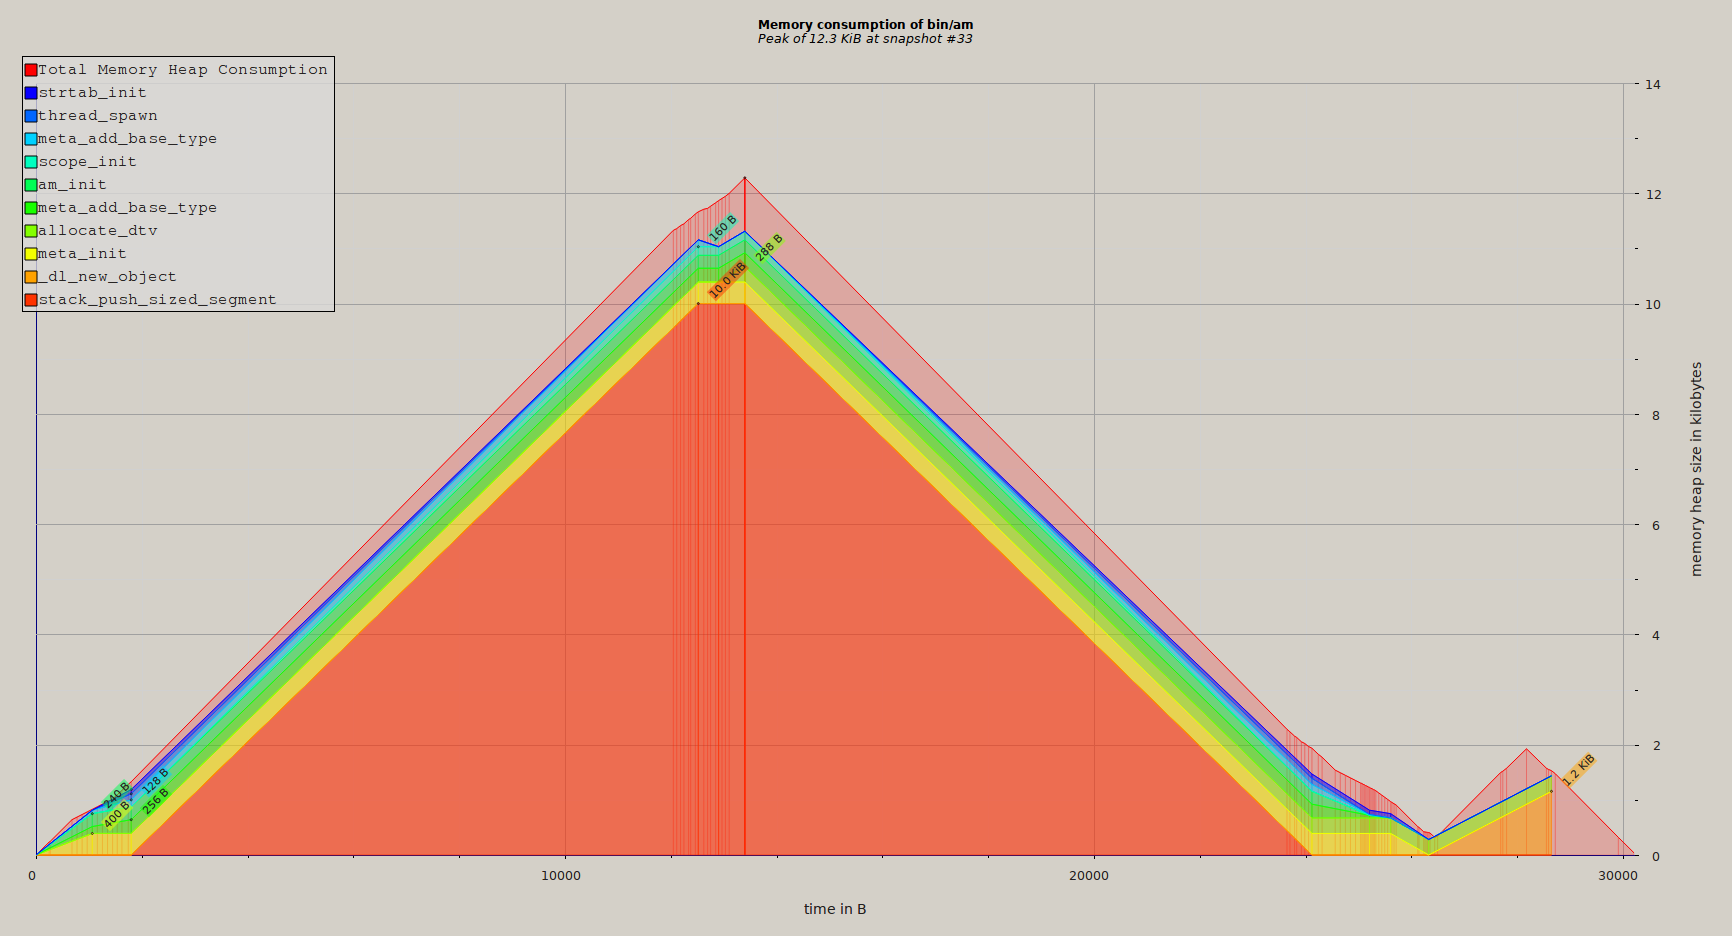
\includegraphics[scale=0.35]{figures/fig-mem}
\end{figure}

\subsubsection{Optimization}

During the majority of the development we did not concern ourselves with
algorithmic optimization, but rather focused on designing suitable data
structures and writing maintainable and concise code that we would be able to
cope with the inevitable changes during the course of the project. As Rob Pike
states it in his first Rule of Programming: ``You can't tell where a program is
going to spend its time. Bottlenecks occur in surprising places, so don't try to
second guess and put in a speed hack until you've proven that's where the
bottleneck is.''\cite{pike-rules}. When the machine had reached a maturity level
that assured us that no further major changes to the overarching design were
necessary we started to analyze the code at a much more detailed level.

Memory leaks are extremely difficult to avoid when writing any non-trivial C
code. One has to meticulously track allocated memory chunks and free them at
just the right time and place to prevent invalid reads and writes. The fact that
C largely does not care about what some collection of bytes represents and
allows virtually any casting does not make this easier. One-off errors are
common when dealing with arrays and pointers which are indeed a central part of
the \thename{} implementation. Luckily there are tools available to aid in
profiling and pinpointing problematic parts of the code. The absolutely
brilliant instrumentation tool Valgrind\footnote{Valgrind:
  \url{http://valgrind.org}} has been an invaluable help for detecting memory
errors and have allowed us to fix, to our knowledge, all problematic leaks.

Valgrind consists of several different tools that analyze different things like
threads, stack operations, caches and memory. We have used the memory error
detector called Memcheck for finding leaks. When an executable is run through
Valgrind it is able to track allocations and the corresponding releases made
during the entire execution. If an allocation does not have exactly one
corresponding free operation it is either a leak or a double free (i.e.~a single
memory region attempted to be released more than once).

The output from Memcheck includes a list of errors and a summary of the leaked
amount of memory. When we initially ran Valgrind with the fibonacci test program
(with $n=15$) the leak summary was this:

\begin{verbatim}
==32067== LEAK SUMMARY:
==32067==    definitely lost: 410,033 bytes in 13,187 blocks
==32067==    indirectly lost: 371,808 bytes in 365 blocks
...
==32067== ERROR SUMMARY: 10 errors from 10 contexts (suppressed: 0 from 0)
\end{verbatim}

This says that there are 10 distinct errors causing a total leak of 400kB
memory, which is a very significant amount of memory for such a small and simple
program. Optimally there should be no bytes leaked at all. Valgrind also tells
you exactly where errors are introduced:

\begin{verbatim}
...
==32067== 27,608 bytes in 986 blocks are definitely lost in loss record 4 of 15
==32067==    at 0x4C29F90: malloc (in /usr/lib/valgrind/vgpreload_memcheck-amd64-linux.so)
==32067==    by 0x4018F4: stack_create_element (stack.c:128)
...
\end{verbatim}

An allocation is being made in the function \code{stack\_create\_element} and is
not released when the program exits. In this case we were not properly releasing
temporary stack elements, and being aware of the issue we changed the way stack
elements are created resulting in a sum total of 40 bytes leaked, all of which
are test data structures that are irrelevant for the actual performance
analysis. It is important to run multiple types of test programs through
Valgrind, because each of them may expose errors in differents parts of the
code.

The other form of profiling we did was by use of the equally great tool called
gprof\footnote{GNU gprof: \url{https://sourceware.org/binutils/docs/gprof/}}
(for GNU profiler). It works in a somewhat different way than Valgrind:
executables are compiled with a special profiling flag that injects profiling
code into the binary. When the file is executed it generates data that is then
run through gprof that performs the analysis. The output is a detailed overview
of the CPU time spent in each function. It is important to avoid profiling
optimized binaries because some crucial information can be lost when the
compiler performs various code transformations. For example, if the compiler
inlines a function into another, the former will appear to be using the
resources that are actually spent by the inlined function.

As an example of how we used gprof to pinpoint bottlenecks, an initial analysis
showed that 9\% of the total running time was spent in the function
\code{bytes2int} which converts a sequence of bytes into an integral C value. It
is a frequent operation but we found it is suspicious to be using almost one
tenth of the total CPU resources. It was indeed not optimally implemented;
Listing~\ref{lst:eval:gprof-pre} and~\ref{lst:eval:gprof-post} shows the
specific code before and after optimization.

\begin{minipage}{\linewidth}
\begin{lstlisting}[language={[ANSI]C},%
  caption={The function \code{bytes2int} before optimization.},%
  label={lst:eval:gprof-pre}]
int64_t value = 0;
int i = size;
while (i) {
    value += ((int64_t) bytes[i - 1]) << (8 * (size - i));
    i--;
}
return value;
\end{lstlisting}

\begin{lstlisting}[language={[ANSI]C},%
  caption={The function \code{bytes2int} after optimization},%
  label={lst:eval:gprof-post}]
switch (size) {
case 1: return bytes[0];
case 2: return bytes[1] | bytes[0] << 8;
case 4: return __builtin_bswap32(*(int32_t*)bytes);
case 8: return __builtin_bswap64(*(int64_t*)bytes);
default: return 0;
}
\end{lstlisting}
\end{minipage}

The optimized version of the function clocked in at the much better 1.4\% CPU
time. Using this technique of measuring, pinpointing, patching and measuring
again we managed to more than triple the speed of some test programs! Currently
the bottleneck of the machine seems to lie somewhere in the stack
implementation, as shown in the following gprof output:

\begin{verbatim}
  %   cumulative   self              self     total
 time   seconds   seconds    calls  ms/call  ms/call  name
 20.24      0.52     0.52 35002981     0.00     0.00  am_exec_instr
  8.17      0.73     0.21 24232831     0.00     0.00  stack_segment_push_element
  6.62      0.90     0.17 35002981     0.00     0.00  am_read_prefixes
  5.64      1.05     0.15 24232831     0.00     0.00  stack_push
  5.06      1.18     0.13 17501491     0.00     0.00  stack_peek
...
\end{verbatim}

Generally it is difficult to determine whether there is a problem with a part of
the code or if it is just a frequent operation in the specific
program. Profiling multiple test programs that utilize different features can
reveal common bottlenecks which should be analyzed further.

Whether there are more fundamental architectural design issues that limits
performance is difficult to say. We have not encountered major issues with how
the modules interoperate.

% JIT

A common form of optimization in modern abstract machines is the process of
compiling a program run-time, rather than prior to execution. This technique is
called just-in-time compilation, or JIT.\@This allows sections of code to be
translated to machine code which the host machine can execute directly. This is
done just before the code is going to be executed, hence the name. The
translated machine code can then be cached and reused. Therefore, if a function
is called multiple times, the machine can save time by paying the overhead of
translating it to machine code, but then saving time every time the same code is
to be executed. A challenge with JITing is balancing the overhead of translating
to machine code versus the saved time during execution. This overhead of
just-in-time compilation is called the ``startup time delay''.

In our earlier performance analysis, we have disabled all forms for such
optimizations to make the execution process of the different machines closer to
that of \thename{}. Figure~\ref{fig:eval:benchmark:jit} shows a benchmark of the
heap workout being run on JVM with and without JIT compilation.

\begin{figure}[H]
  \centering
  \scalebox{0.8}[0.6]{% Created by tikzDevice version 0.8.1 on 2015-06-28 21:11:30
% !TEX encoding = UTF-8 Unicode
\begin{tikzpicture}[x=1pt,y=1pt]
\definecolor{fillColor}{RGB}{255,255,255}
\path[use as bounding box,fill=fillColor,fill opacity=0.00] (0,0) rectangle (505.89,505.89);
\begin{scope}
\path[clip] (  0.00,  0.00) rectangle (505.89,505.89);
\definecolor{drawColor}{RGB}{255,255,255}
\definecolor{fillColor}{RGB}{255,255,255}

\path[draw=drawColor,line width= 0.6pt,line join=round,line cap=round,fill=fillColor] (  0.00,  0.00) rectangle (505.89,505.89);
\end{scope}
\begin{scope}
\path[clip] ( 32.22, 35.66) rectangle (420.79,493.85);
\definecolor{fillColor}{gray}{0.90}

\path[fill=fillColor] ( 32.22, 35.66) rectangle (420.79,493.85);
\definecolor{drawColor}{gray}{0.95}

\path[draw=drawColor,line width= 0.3pt,line join=round] ( 32.22,109.17) --
	(420.79,109.17);

\path[draw=drawColor,line width= 0.3pt,line join=round] ( 32.22,214.53) --
	(420.79,214.53);

\path[draw=drawColor,line width= 0.3pt,line join=round] ( 32.22,319.89) --
	(420.79,319.89);

\path[draw=drawColor,line width= 0.3pt,line join=round] ( 32.22,425.25) --
	(420.79,425.25);

\path[draw=drawColor,line width= 0.3pt,line join=round] ( 85.80, 35.66) --
	( 85.80,493.85);

\path[draw=drawColor,line width= 0.3pt,line join=round] (157.62, 35.66) --
	(157.62,493.85);

\path[draw=drawColor,line width= 0.3pt,line join=round] (229.44, 35.66) --
	(229.44,493.85);

\path[draw=drawColor,line width= 0.3pt,line join=round] (301.27, 35.66) --
	(301.27,493.85);

\path[draw=drawColor,line width= 0.3pt,line join=round] (373.09, 35.66) --
	(373.09,493.85);
\definecolor{drawColor}{RGB}{255,255,255}

\path[draw=drawColor,line width= 0.6pt,line join=round] ( 32.22, 56.49) --
	(420.79, 56.49);

\path[draw=drawColor,line width= 0.6pt,line join=round] ( 32.22,161.85) --
	(420.79,161.85);

\path[draw=drawColor,line width= 0.6pt,line join=round] ( 32.22,267.21) --
	(420.79,267.21);

\path[draw=drawColor,line width= 0.6pt,line join=round] ( 32.22,372.57) --
	(420.79,372.57);

\path[draw=drawColor,line width= 0.6pt,line join=round] ( 32.22,477.94) --
	(420.79,477.94);

\path[draw=drawColor,line width= 0.6pt,line join=round] ( 49.88, 35.66) --
	( 49.88,493.85);

\path[draw=drawColor,line width= 0.6pt,line join=round] (121.71, 35.66) --
	(121.71,493.85);

\path[draw=drawColor,line width= 0.6pt,line join=round] (193.53, 35.66) --
	(193.53,493.85);

\path[draw=drawColor,line width= 0.6pt,line join=round] (265.36, 35.66) --
	(265.36,493.85);

\path[draw=drawColor,line width= 0.6pt,line join=round] (337.18, 35.66) --
	(337.18,493.85);

\path[draw=drawColor,line width= 0.6pt,line join=round] (409.00, 35.66) --
	(409.00,493.85);
\definecolor{drawColor}{RGB}{248,118,109}

\path[draw=drawColor,line width= 0.6pt,line join=round] ( 49.88, 64.92) --
	(342.43, 73.70) --
	(353.24, 80.72) --
	(359.56, 88.45) --
	(364.05, 97.23) --
	(367.53,102.14) --
	(370.37,111.63) --
	(372.78,122.86) --
	(374.86,124.62) --
	(376.70,131.29) --
	(378.34,140.07) --
	(379.82,151.66) --
	(381.18,154.47) --
	(382.43,163.96) --
	(383.59,170.98) --
	(384.66,174.14) --
	(385.67,183.97) --
	(386.61,191.00) --
	(387.51,200.83) --
	(388.35,232.09) --
	(389.15,237.01) --
	(389.91,236.30) --
	(390.64,233.14) --
	(391.33,231.39) --
	(391.99,251.76) --
	(392.63,255.27) --
	(393.24,257.38) --
	(393.83,261.94) --
	(394.40,266.86) --
	(394.94,280.91) --
	(395.47,291.80) --
	(395.98,293.55) --
	(396.48,301.98) --
	(396.96,320.24) --
	(397.42,338.86) --
	(397.88,336.40) --
	(398.32,357.47) --
	(398.74,339.56) --
	(399.16,350.10) --
	(399.56,367.30) --
	(399.96,399.97) --
	(400.34,411.91) --
	(400.72,415.77) --
	(401.09,417.88) --
	(401.45,433.33) --
	(401.80,468.10) --
	(402.14,473.02) --
	(402.47,444.57) --
	(402.80,416.12) --
	(403.12,417.53);
\definecolor{drawColor}{RGB}{0,191,196}

\path[draw=drawColor,line width= 0.6pt,line join=round] ( 49.88, 66.67) --
	(282.49, 73.70) --
	(293.30, 80.37) --
	(299.62, 87.39) --
	(304.11, 94.07) --
	(307.59,101.44) --
	(310.43,115.49) --
	(312.84,115.14) --
	(314.92,121.46) --
	(316.76,130.59) --
	(318.40,139.72) --
	(319.89,144.29) --
	(321.24,151.66) --
	(322.49,156.58) --
	(323.65,166.41) --
	(324.73,170.63) --
	(325.73,179.76) --
	(326.68,190.65) --
	(327.57,209.26) --
	(328.41,202.24) --
	(329.21,208.91) --
	(329.97,215.93) --
	(330.70,222.96) --
	(331.39,227.17) --
	(332.06,236.30) --
	(332.69,243.33) --
	(333.30,248.60) --
	(333.89,257.38) --
	(334.46,263.35) --
	(335.01,268.26) --
	(335.54,277.40) --
	(336.05,289.69) --
	(336.54,290.39) --
	(337.02,303.03) --
	(337.49,305.49) --
	(337.94,312.17) --
	(338.38,320.59) --
	(338.81,328.67) --
	(339.22,334.64) --
	(339.63,340.26) --
	(340.02,350.80) --
	(340.41,353.26) --
	(340.78,373.28) --
	(341.15,390.84) --
	(341.51,385.22) --
	(341.86,418.23) --
	(342.20,444.92) --
	(342.54,440.00) --
	(342.87,414.02) --
	(343.19,429.12);
\end{scope}
\begin{scope}
\path[clip] (  0.00,  0.00) rectangle (505.89,505.89);
\definecolor{drawColor}{gray}{0.50}

\node[text=drawColor,anchor=base east,inner sep=0pt, outer sep=0pt, scale=  0.96] at ( 25.11, 53.18) {0};

\node[text=drawColor,anchor=base east,inner sep=0pt, outer sep=0pt, scale=  0.96] at ( 25.11,158.54) {1};

\node[text=drawColor,anchor=base east,inner sep=0pt, outer sep=0pt, scale=  0.96] at ( 25.11,263.90) {2};

\node[text=drawColor,anchor=base east,inner sep=0pt, outer sep=0pt, scale=  0.96] at ( 25.11,369.27) {3};

\node[text=drawColor,anchor=base east,inner sep=0pt, outer sep=0pt, scale=  0.96] at ( 25.11,474.63) {4};
\end{scope}
\begin{scope}
\path[clip] (  0.00,  0.00) rectangle (505.89,505.89);
\definecolor{drawColor}{gray}{0.50}

\path[draw=drawColor,line width= 0.6pt,line join=round] ( 27.95, 56.49) --
	( 32.22, 56.49);

\path[draw=drawColor,line width= 0.6pt,line join=round] ( 27.95,161.85) --
	( 32.22,161.85);

\path[draw=drawColor,line width= 0.6pt,line join=round] ( 27.95,267.21) --
	( 32.22,267.21);

\path[draw=drawColor,line width= 0.6pt,line join=round] ( 27.95,372.57) --
	( 32.22,372.57);

\path[draw=drawColor,line width= 0.6pt,line join=round] ( 27.95,477.94) --
	( 32.22,477.94);
\end{scope}
\begin{scope}
\path[clip] (  0.00,  0.00) rectangle (505.89,505.89);
\definecolor{drawColor}{gray}{0.50}

\path[draw=drawColor,line width= 0.6pt,line join=round] ( 49.88, 31.39) --
	( 49.88, 35.66);

\path[draw=drawColor,line width= 0.6pt,line join=round] (121.71, 31.39) --
	(121.71, 35.66);

\path[draw=drawColor,line width= 0.6pt,line join=round] (193.53, 31.39) --
	(193.53, 35.66);

\path[draw=drawColor,line width= 0.6pt,line join=round] (265.36, 31.39) --
	(265.36, 35.66);

\path[draw=drawColor,line width= 0.6pt,line join=round] (337.18, 31.39) --
	(337.18, 35.66);

\path[draw=drawColor,line width= 0.6pt,line join=round] (409.00, 31.39) --
	(409.00, 35.66);
\end{scope}
\begin{scope}
\path[clip] (  0.00,  0.00) rectangle (505.89,505.89);
\definecolor{drawColor}{gray}{0.50}

\node[text=drawColor,anchor=base west,inner sep=0pt, outer sep=0pt, scale=  0.96] at ( 43.41, 20.31) {10};

\node[text=drawColor,anchor=base west,inner sep=0pt, outer sep=0pt, scale=  0.67] at ( 53.00, 24.24) {0};

\node[text=drawColor,anchor=base west,inner sep=0pt, outer sep=0pt, scale=  0.96] at (115.23, 20.31) {10};

\node[text=drawColor,anchor=base west,inner sep=0pt, outer sep=0pt, scale=  0.67] at (124.83, 24.24) {2};

\node[text=drawColor,anchor=base west,inner sep=0pt, outer sep=0pt, scale=  0.96] at (187.05, 20.31) {10};

\node[text=drawColor,anchor=base west,inner sep=0pt, outer sep=0pt, scale=  0.67] at (196.65, 24.24) {4};

\node[text=drawColor,anchor=base west,inner sep=0pt, outer sep=0pt, scale=  0.96] at (258.88, 20.31) {10};

\node[text=drawColor,anchor=base west,inner sep=0pt, outer sep=0pt, scale=  0.67] at (268.47, 24.24) {6};

\node[text=drawColor,anchor=base west,inner sep=0pt, outer sep=0pt, scale=  0.96] at (330.70, 20.31) {10};

\node[text=drawColor,anchor=base west,inner sep=0pt, outer sep=0pt, scale=  0.67] at (340.30, 24.24) {8};

\node[text=drawColor,anchor=base west,inner sep=0pt, outer sep=0pt, scale=  0.96] at (400.84, 20.31) {10};

\node[text=drawColor,anchor=base west,inner sep=0pt, outer sep=0pt, scale=  0.67] at (410.44, 24.24) {1};

\node[text=drawColor,anchor=base west,inner sep=0pt, outer sep=0pt, scale=  0.67] at (413.80, 24.24) {0};
\end{scope}
\begin{scope}
\path[clip] (  0.00,  0.00) rectangle (505.89,505.89);
\definecolor{drawColor}{RGB}{0,0,0}

\node[text=drawColor,anchor=base,inner sep=0pt, outer sep=0pt, scale=  1.20] at (226.50,  9.03) {n};
\end{scope}
\begin{scope}
\path[clip] (  0.00,  0.00) rectangle (505.89,505.89);
\definecolor{drawColor}{RGB}{0,0,0}

\node[text=drawColor,rotate= 90.00,anchor=base,inner sep=0pt, outer sep=0pt, scale=  1.20] at ( 17.30,264.75) {Mean-time};
\end{scope}
\begin{scope}
\path[clip] (  0.00,  0.00) rectangle (505.89,505.89);
\definecolor{fillColor}{RGB}{255,255,255}

\path[fill=fillColor] (429.65,240.91) rectangle (484.98,288.59);
\end{scope}
\begin{scope}
\path[clip] (  0.00,  0.00) rectangle (505.89,505.89);
\definecolor{drawColor}{RGB}{0,0,0}

\node[text=drawColor,anchor=base west,inner sep=0pt, outer sep=0pt, scale=  0.96] at (433.92,277.70) {\bfseries Machine};
\end{scope}
\begin{scope}
\path[clip] (  0.00,  0.00) rectangle (505.89,505.89);
\definecolor{drawColor}{RGB}{255,255,255}
\definecolor{fillColor}{gray}{0.95}

\path[draw=drawColor,line width= 0.6pt,line join=round,line cap=round,fill=fillColor] (433.92,259.63) rectangle (448.38,274.09);
\end{scope}
\begin{scope}
\path[clip] (  0.00,  0.00) rectangle (505.89,505.89);
\definecolor{drawColor}{RGB}{248,118,109}

\path[draw=drawColor,line width= 0.6pt,line join=round] (435.37,266.86) -- (446.93,266.86);
\end{scope}
\begin{scope}
\path[clip] (  0.00,  0.00) rectangle (505.89,505.89);
\definecolor{drawColor}{RGB}{255,255,255}
\definecolor{fillColor}{gray}{0.95}

\path[draw=drawColor,line width= 0.6pt,line join=round,line cap=round,fill=fillColor] (433.92,245.18) rectangle (448.38,259.63);
\end{scope}
\begin{scope}
\path[clip] (  0.00,  0.00) rectangle (505.89,505.89);
\definecolor{drawColor}{RGB}{0,191,196}

\path[draw=drawColor,line width= 0.6pt,line join=round] (435.37,252.41) -- (446.93,252.41);
\end{scope}
\begin{scope}
\path[clip] (  0.00,  0.00) rectangle (505.89,505.89);
\definecolor{drawColor}{RGB}{0,0,0}

\node[text=drawColor,anchor=base west,inner sep=0pt, outer sep=0pt, scale=  0.96] at (450.18,263.55) {JIT};
\end{scope}
\begin{scope}
\path[clip] (  0.00,  0.00) rectangle (505.89,505.89);
\definecolor{drawColor}{RGB}{0,0,0}

\node[text=drawColor,anchor=base west,inner sep=0pt, outer sep=0pt, scale=  0.96] at (450.18,249.10) {No JIT};
\end{scope}
\end{tikzpicture}
}
  \caption{JIT comparing on JVM}
\label{fig:eval:benchmark:jit}
\end{figure}

The benefit of JIT compilation is striking, it runs more than an order of
magnitude faster. Even with small numbers, we see that the statup time delay
that occurs when using JIT is still outweighed by the faster execution
time. This is obviously a very simple program which means that the JIT process
will be very short, and thus the cost of JITting is most certainly higher for
larger programs.

\subsection{Code Analysis}

Another side of code evaluation is to view the source code from a macro
perspective, including trivial things such as counting source lines of code
(SLOC) and looking at the number of comments per line of
code. Figure~\ref{fig:eval:sloc} shows the division of code in the source
directory and in the tests. The amount of source code is well correlated with
the amount of work performed by each module. The test SLOC are not proportional
to the amount of code in the corresponding module because some algorithms
require much more extensive unit tests than others. For instance the type
conversion algorithms must cover almost all different combinations of types
which results in extensive tests.

\begin{figure}
  \centering
  % Created by tikzDevice version 0.8.1 on 2015-06-28 21:35:40
% !TEX encoding = UTF-8 Unicode
\begin{tikzpicture}[x=1pt,y=1pt]
\definecolor{fillColor}{RGB}{255,255,255}
\path[use as bounding box,fill=fillColor,fill opacity=0.00] (0,0) rectangle (505.89,505.89);
\begin{scope}
\path[clip] ( 49.20,314.14) rectangle (480.69,456.69);
\definecolor{drawColor}{RGB}{0,0,0}
\definecolor{fillColor}{RGB}{255,255,255}

\path[draw=drawColor,line width= 0.4pt,line join=round,line cap=round,fill=fillColor] (330.94,385.42) --
	(330.90,387.64) --
	(330.79,389.87) --
	(330.60,392.09) --
	(330.34,394.30) --
	(330.00,396.50) --
	(329.59,398.69) --
	(329.10,400.87) --
	(328.55,403.02) --
	(327.92,405.16) --
	(327.21,407.27) --
	(326.44,409.36) --
	(325.60,411.43) --
	(324.68,413.46) --
	(323.70,415.46) --
	(322.66,417.42) --
	(321.54,419.35) --
	(320.37,421.24) --
	(319.13,423.09) --
	(317.82,424.90) --
	(316.46,426.66) --
	(315.04,428.38) --
	(264.94,385.42) --
	cycle;

\path[draw=drawColor,line width= 0.4pt,line join=round,line cap=round] (326.84,408.32) --
	(329.93,409.47);
\end{scope}
\begin{scope}
\path[clip] (  0.00,252.94) rectangle (505.89,505.89);
\definecolor{drawColor}{RGB}{0,0,0}

\node[text=drawColor,anchor=base west,inner sep=0pt, outer sep=0pt, scale=  1.00] at (333.02,408.14) {engine+rtl};
\end{scope}
\begin{scope}
\path[clip] ( 49.20,314.14) rectangle (480.69,456.69);
\definecolor{drawColor}{RGB}{0,0,0}
\definecolor{fillColor}{RGB}{173,216,230}

\path[draw=drawColor,line width= 0.4pt,line join=round,line cap=round,fill=fillColor] (315.04,428.38) --
	(313.60,430.00) --
	(312.10,431.58) --
	(310.56,433.11) --
	(308.96,434.58) --
	(307.32,436.01) --
	(305.63,437.37) --
	(303.90,438.68) --
	(302.13,439.94) --
	(300.31,441.13) --
	(298.46,442.27) --
	(296.57,443.34) --
	(294.65,444.35) --
	(292.69,445.29) --
	(290.71,446.17) --
	(288.69,446.99) --
	(286.65,447.74) --
	(284.59,448.42) --
	(282.51,449.03) --
	(280.40,449.57) --
	(278.28,450.05) --
	(276.15,450.45) --
	(274.00,450.79) --
	(271.85,451.05) --
	(269.68,451.24) --
	(267.51,451.36) --
	(265.34,451.41) --
	(263.17,451.39) --
	(261.00,451.29) --
	(258.83,451.13) --
	(256.67,450.89) --
	(254.52,450.58) --
	(252.38,450.20) --
	(250.26,449.76) --
	(248.15,449.24) --
	(246.06,448.65) --
	(243.99,447.99) --
	(241.94,447.27) --
	(239.91,446.48) --
	(237.92,445.62) --
	(235.95,444.70) --
	(234.02,443.71) --
	(264.94,385.42) --
	cycle;

\path[draw=drawColor,line width= 0.4pt,line join=round,line cap=round] (277.22,450.26) --
	(277.83,453.50);
\end{scope}
\begin{scope}
\path[clip] (  0.00,252.94) rectangle (505.89,505.89);
\definecolor{drawColor}{RGB}{0,0,0}

\node[text=drawColor,anchor=base west,inner sep=0pt, outer sep=0pt, scale=  1.00] at (278.44,453.43) {instructions};
\end{scope}
\begin{scope}
\path[clip] ( 49.20,314.14) rectangle (480.69,456.69);
\definecolor{drawColor}{RGB}{0,0,0}
\definecolor{fillColor}{RGB}{255,228,225}

\path[draw=drawColor,line width= 0.4pt,line join=round,line cap=round,fill=fillColor] (234.02,443.71) --
	(232.08,442.64) --
	(230.17,441.51) --
	(228.31,440.31) --
	(226.49,439.05) --
	(224.71,437.72) --
	(222.97,436.34) --
	(221.28,434.90) --
	(219.65,433.41) --
	(218.06,431.86) --
	(216.53,430.26) --
	(215.05,428.61) --
	(213.63,426.91) --
	(212.26,425.16) --
	(210.96,423.37) --
	(209.71,421.53) --
	(208.53,419.66) --
	(207.41,417.75) --
	(206.36,415.79) --
	(205.37,413.81) --
	(204.45,411.79) --
	(203.60,409.75) --
	(202.82,407.67) --
	(264.94,385.42) --
	cycle;

\path[draw=drawColor,line width= 0.4pt,line join=round,line cap=round] (215.05,428.61) --
	(212.55,430.77);
\end{scope}
\begin{scope}
\path[clip] (  0.00,252.94) rectangle (505.89,505.89);
\definecolor{drawColor}{RGB}{0,0,0}

\node[text=drawColor,anchor=base east,inner sep=0pt, outer sep=0pt, scale=  1.00] at (210.06,430.78) {am};
\end{scope}
\begin{scope}
\path[clip] ( 49.20,314.14) rectangle (480.69,456.69);
\definecolor{drawColor}{RGB}{0,0,0}
\definecolor{fillColor}{RGB}{224,255,255}

\path[draw=drawColor,line width= 0.4pt,line join=round,line cap=round,fill=fillColor] (202.82,407.67) --
	(202.09,405.53) --
	(201.44,403.36) --
	(200.86,401.18) --
	(200.36,398.97) --
	(199.93,396.75) --
	(199.58,394.52) --
	(199.31,392.27) --
	(199.11,390.02) --
	(198.99,387.76) --
	(198.95,385.50) --
	(198.99,383.24) --
	(199.10,380.98) --
	(199.29,378.73) --
	(264.94,385.42) --
	cycle;

\path[draw=drawColor,line width= 0.4pt,line join=round,line cap=round] (199.44,393.40) --
	(196.16,393.80);
\end{scope}
\begin{scope}
\path[clip] (  0.00,252.94) rectangle (505.89,505.89);
\definecolor{drawColor}{RGB}{0,0,0}

\node[text=drawColor,anchor=base east,inner sep=0pt, outer sep=0pt, scale=  1.00] at (192.89,390.75) {stack};
\end{scope}
\begin{scope}
\path[clip] ( 49.20,314.14) rectangle (480.69,456.69);
\definecolor{drawColor}{RGB}{0,0,0}
\definecolor{fillColor}{RGB}{230,230,250}

\path[draw=drawColor,line width= 0.4pt,line join=round,line cap=round,fill=fillColor] (199.29,378.73) --
	(199.57,376.40) --
	(199.93,374.08) --
	(200.38,371.78) --
	(200.90,369.49) --
	(201.51,367.23) --
	(202.20,364.98) --
	(202.96,362.77) --
	(203.81,360.58) --
	(264.94,385.42) --
	cycle;

\path[draw=drawColor,line width= 0.4pt,line join=round,line cap=round] (200.90,369.49) --
	(197.70,368.70);
\end{scope}
\begin{scope}
\path[clip] (  0.00,252.94) rectangle (505.89,505.89);
\definecolor{drawColor}{RGB}{0,0,0}

\node[text=drawColor,anchor=base east,inner sep=0pt, outer sep=0pt, scale=  1.00] at (194.50,364.46) {thread};
\end{scope}
\begin{scope}
\path[clip] ( 49.20,314.14) rectangle (480.69,456.69);
\definecolor{drawColor}{RGB}{0,0,0}
\definecolor{fillColor}{RGB}{255,248,220}

\path[draw=drawColor,line width= 0.4pt,line join=round,line cap=round,fill=fillColor] (203.81,360.58) --
	(204.89,358.06) --
	(206.07,355.60) --
	(207.36,353.18) --
	(208.75,350.82) --
	(210.23,348.52) --
	(211.81,346.28) --
	(264.94,385.42) --
	cycle;

\path[draw=drawColor,line width= 0.4pt,line join=round,line cap=round] (207.36,353.18) --
	(204.48,351.57);
\end{scope}
\begin{scope}
\path[clip] (  0.00,252.94) rectangle (505.89,505.89);
\definecolor{drawColor}{RGB}{0,0,0}

\node[text=drawColor,anchor=base east,inner sep=0pt, outer sep=0pt, scale=  1.00] at (201.60,347.48) {gc+loader};
\end{scope}
\begin{scope}
\path[clip] ( 49.20,314.14) rectangle (480.69,456.69);
\definecolor{drawColor}{RGB}{0,0,0}
\definecolor{fillColor}{RGB}{255,255,255}

\path[draw=drawColor,line width= 0.4pt,line join=round,line cap=round,fill=fillColor] (211.81,346.28) --
	(213.12,344.57) --
	(214.48,342.90) --
	(215.89,341.27) --
	(217.35,339.70) --
	(218.87,338.17) --
	(220.44,336.69) --
	(222.05,335.27) --
	(223.71,333.89) --
	(225.41,332.58) --
	(227.15,331.32) --
	(228.94,330.11) --
	(230.76,328.97) --
	(232.62,327.88) --
	(234.51,326.86) --
	(236.44,325.90) --
	(238.40,325.00) --
	(240.38,324.17) --
	(242.39,323.40) --
	(244.43,322.70) --
	(246.48,322.06) --
	(248.56,321.49) --
	(250.65,320.99) --
	(252.76,320.56) --
	(254.88,320.20) --
	(257.02,319.90) --
	(259.16,319.68) --
	(261.30,319.52) --
	(263.46,319.44) --
	(265.61,319.43) --
	(267.76,319.48) --
	(269.91,319.61) --
	(272.05,319.81) --
	(274.19,320.07) --
	(276.31,320.41) --
	(278.43,320.82) --
	(280.53,321.29) --
	(282.61,321.83) --
	(284.68,322.44) --
	(286.72,323.12) --
	(288.74,323.86) --
	(290.73,324.67) --
	(292.70,325.55) --
	(294.64,326.48) --
	(296.55,327.48) --
	(298.42,328.54) --
	(300.26,329.67) --
	(302.05,330.85) --
	(264.94,385.42) --
	cycle;

\path[draw=drawColor,line width= 0.4pt,line join=round,line cap=round] (253.82,320.37) --
	(253.27,317.12);
\end{scope}
\begin{scope}
\path[clip] (  0.00,252.94) rectangle (505.89,505.89);
\definecolor{drawColor}{RGB}{0,0,0}

\node[text=drawColor,anchor=base east,inner sep=0pt, outer sep=0pt, scale=  1.00] at (252.71,311.39) {info tables+types};
\end{scope}
\begin{scope}
\path[clip] ( 49.20,314.14) rectangle (480.69,456.69);
\definecolor{drawColor}{RGB}{0,0,0}
\definecolor{fillColor}{RGB}{173,216,230}

\path[draw=drawColor,line width= 0.4pt,line join=round,line cap=round,fill=fillColor] (302.05,330.85) --
	(303.87,332.12) --
	(305.63,333.46) --
	(307.35,334.85) --
	(309.03,336.31) --
	(310.65,337.81) --
	(312.22,339.37) --
	(313.74,340.99) --
	(315.21,342.65) --
	(316.61,344.36) --
	(317.96,346.12) --
	(319.25,347.92) --
	(320.48,349.76) --
	(321.64,351.65) --
	(322.75,353.57) --
	(323.78,355.53) --
	(324.75,357.52) --
	(325.65,359.54) --
	(326.49,361.60) --
	(327.25,363.68) --
	(327.95,365.78) --
	(328.57,367.91) --
	(329.12,370.05) --
	(329.60,372.21) --
	(330.01,374.39) --
	(330.34,376.58) --
	(330.60,378.78) --
	(330.79,380.99) --
	(330.90,383.20) --
	(330.94,385.42) --
	(264.94,385.42) --
	cycle;

\path[draw=drawColor,line width= 0.4pt,line join=round,line cap=round] (323.27,354.55) --
	(326.19,353.00);
\end{scope}
\begin{scope}
\path[clip] (  0.00,252.94) rectangle (505.89,505.89);
\definecolor{drawColor}{RGB}{0,0,0}

\node[text=drawColor,anchor=base west,inner sep=0pt, outer sep=0pt, scale=  1.00] at (329.10,348.99) {utils and debugging};

\node[text=drawColor,anchor=base,inner sep=0pt, outer sep=0pt, scale=  1.20] at (264.94,477.15) {\bfseries SLOC per module};
\end{scope}
\begin{scope}
\path[clip] ( 49.20, 61.20) rectangle (480.69,203.75);
\definecolor{drawColor}{RGB}{0,0,0}
\definecolor{fillColor}{RGB}{255,255,255}

\path[draw=drawColor,line width= 0.4pt,line join=round,line cap=round,fill=fillColor] (330.94,132.47) --
	(330.90,134.64) --
	(330.80,136.81) --
	(330.62,138.97) --
	(330.37,141.12) --
	(330.05,143.27) --
	(329.66,145.40) --
	(329.20,147.52) --
	(328.67,149.62) --
	(328.07,151.70) --
	(327.41,153.77) --
	(326.67,155.81) --
	(325.87,157.82) --
	(325.01,159.81) --
	(324.08,161.77) --
	(323.08,163.70) --
	(322.03,165.59) --
	(320.91,167.45) --
	(319.73,169.27) --
	(318.49,171.05) --
	(317.19,172.78) --
	(315.84,174.48) --
	(314.44,176.13) --
	(312.97,177.73) --
	(311.46,179.28) --
	(309.90,180.79) --
	(308.29,182.24) --
	(306.63,183.63) --
	(304.93,184.98) --
	(303.18,186.26) --
	(264.94,132.47) --
	cycle;

\path[draw=drawColor,line width= 0.4pt,line join=round,line cap=round] (323.59,162.74) --
	(326.52,164.25);
\end{scope}
\begin{scope}
\path[clip] (  0.00,  0.00) rectangle (505.89,252.94);
\definecolor{drawColor}{RGB}{0,0,0}

\node[text=drawColor,anchor=base west,inner sep=0pt, outer sep=0pt, scale=  1.00] at (329.45,163.29) {engine+rtl};
\end{scope}
\begin{scope}
\path[clip] ( 49.20, 61.20) rectangle (480.69,203.75);
\definecolor{drawColor}{RGB}{0,0,0}
\definecolor{fillColor}{RGB}{173,216,230}

\path[draw=drawColor,line width= 0.4pt,line join=round,line cap=round,fill=fillColor] (303.18,186.26) --
	(301.23,187.59) --
	(299.24,188.86) --
	(297.20,190.05) --
	(295.12,191.17) --
	(293.00,192.21) --
	(290.84,193.17) --
	(288.65,194.06) --
	(286.43,194.87) --
	(284.19,195.60) --
	(281.92,196.25) --
	(279.62,196.81) --
	(277.31,197.30) --
	(264.94,132.47) --
	cycle;

\path[draw=drawColor,line width= 0.4pt,line join=round,line cap=round] (290.84,193.17) --
	(292.14,196.21);
\end{scope}
\begin{scope}
\path[clip] (  0.00,  0.00) rectangle (505.89,252.94);
\definecolor{drawColor}{RGB}{0,0,0}

\node[text=drawColor,anchor=base west,inner sep=0pt, outer sep=0pt, scale=  1.00] at (293.43,195.93) {instructions};
\end{scope}
\begin{scope}
\path[clip] ( 49.20, 61.20) rectangle (480.69,203.75);
\definecolor{drawColor}{RGB}{0,0,0}
\definecolor{fillColor}{RGB}{255,228,225}

\path[draw=drawColor,line width= 0.4pt,line join=round,line cap=round,fill=fillColor] (277.31,197.30) --
	(275.21,197.66) --
	(273.09,197.96) --
	(270.97,198.19) --
	(268.84,198.35) --
	(266.71,198.44) --
	(264.57,198.46) --
	(262.43,198.42) --
	(260.30,198.30) --
	(258.17,198.12) --
	(256.05,197.86) --
	(253.94,197.54) --
	(251.84,197.15) --
	(249.75,196.69) --
	(247.68,196.17) --
	(245.63,195.58) --
	(243.60,194.92) --
	(241.59,194.19) --
	(239.60,193.41) --
	(237.64,192.55) --
	(235.71,191.64) --
	(233.81,190.66) --
	(231.95,189.62) --
	(230.11,188.52) --
	(228.32,187.37) --
	(226.56,186.15) --
	(224.84,184.88) --
	(223.17,183.56) --
	(221.54,182.18) --
	(219.95,180.75) --
	(218.41,179.27) --
	(216.92,177.74) --
	(215.48,176.16) --
	(214.09,174.53) --
	(212.76,172.87) --
	(211.48,171.16) --
	(210.25,169.40) --
	(209.09,167.61) --
	(207.98,165.79) --
	(206.93,163.93) --
	(205.94,162.03) --
	(205.02,160.11) --
	(204.15,158.15) --
	(203.35,156.17) --
	(202.62,154.17) --
	(201.95,152.14) --
	(201.35,150.09) --
	(200.81,148.02) --
	(200.34,145.94) --
	(199.94,143.84) --
	(199.60,141.73) --
	(199.34,139.61) --
	(199.14,137.48) --
	(199.01,135.35) --
	(198.96,133.21) --
	(198.97,131.08) --
	(199.05,128.94) --
	(199.20,126.81) --
	(199.41,124.69) --
	(199.70,122.57) --
	(264.94,132.47) --
	cycle;

\path[draw=drawColor,line width= 0.4pt,line join=round,line cap=round] (219.17,180.01) --
	(216.89,182.39);
\end{scope}
\begin{scope}
\path[clip] (  0.00,  0.00) rectangle (505.89,252.94);
\definecolor{drawColor}{RGB}{0,0,0}

\node[text=drawColor,anchor=base east,inner sep=0pt, outer sep=0pt, scale=  1.00] at (214.60,182.61) {am};
\end{scope}
\begin{scope}
\path[clip] ( 49.20, 61.20) rectangle (480.69,203.75);
\definecolor{drawColor}{RGB}{0,0,0}
\definecolor{fillColor}{RGB}{224,255,255}

\path[draw=drawColor,line width= 0.4pt,line join=round,line cap=round,fill=fillColor] (199.70,122.57) --
	(200.05,120.46) --
	(200.48,118.36) --
	(200.97,116.27) --
	(201.53,114.20) --
	(202.16,112.15) --
	(202.85,110.13) --
	(203.61,108.12) --
	(204.43,106.14) --
	(205.32,104.19) --
	(206.27,102.27) --
	(207.28,100.38) --
	(208.35, 98.53) --
	(209.48, 96.71) --
	(210.67, 94.92) --
	(211.92, 93.18) --
	(213.23, 91.48) --
	(214.58, 89.82) --
	(216.00, 88.21) --
	(217.46, 86.65) --
	(218.97, 85.13) --
	(220.53, 83.66) --
	(222.14, 82.24) --
	(223.79, 80.88) --
	(225.49, 79.57) --
	(227.23, 78.32) --
	(229.01, 77.12) --
	(230.82, 75.99) --
	(232.68, 74.91) --
	(234.56, 73.89) --
	(236.48, 72.93) --
	(264.94,132.47) --
	cycle;

\path[draw=drawColor,line width= 0.4pt,line join=round,line cap=round] (211.92, 93.18) --
	(209.27, 91.22);
\end{scope}
\begin{scope}
\path[clip] (  0.00,  0.00) rectangle (505.89,252.94);
\definecolor{drawColor}{RGB}{0,0,0}

\node[text=drawColor,anchor=base east,inner sep=0pt, outer sep=0pt, scale=  1.00] at (206.62, 85.81) {stack};
\end{scope}
\begin{scope}
\path[clip] ( 49.20, 61.20) rectangle (480.69,203.75);
\definecolor{drawColor}{RGB}{0,0,0}
\definecolor{fillColor}{RGB}{230,230,250}

\path[draw=drawColor,line width= 0.4pt,line join=round,line cap=round,fill=fillColor] (236.48, 72.93) --
	(239.10, 71.75) --
	(241.77, 70.68) --
	(244.48, 69.73) --
	(247.24, 68.90) --
	(250.02, 68.19) --
	(264.94,132.47) --
	cycle;

\path[draw=drawColor,line width= 0.4pt,line join=round,line cap=round] (243.12, 70.19) --
	(242.03, 67.08);
\end{scope}
\begin{scope}
\path[clip] (  0.00,  0.00) rectangle (505.89,252.94);
\definecolor{drawColor}{RGB}{0,0,0}

\node[text=drawColor,anchor=base east,inner sep=0pt, outer sep=0pt, scale=  1.00] at (240.94, 60.52) {thread};
\end{scope}
\begin{scope}
\path[clip] ( 49.20, 61.20) rectangle (480.69,203.75);
\definecolor{drawColor}{RGB}{0,0,0}
\definecolor{fillColor}{RGB}{255,248,220}

\path[draw=drawColor,line width= 0.4pt,line join=round,line cap=round,fill=fillColor] (250.02, 68.19) --
	(252.62, 67.64) --
	(255.23, 67.20) --
	(257.86, 66.86) --
	(260.50, 66.63) --
	(263.15, 66.50) --
	(264.94,132.47) --
	cycle;

\path[draw=drawColor,line width= 0.4pt,line join=round,line cap=round] (256.54, 67.02) --
	(256.12, 63.74);
\end{scope}
\begin{scope}
\path[clip] (  0.00,  0.00) rectangle (505.89,252.94);
\definecolor{drawColor}{RGB}{0,0,0}

\node[text=drawColor,anchor=base east,inner sep=0pt, outer sep=0pt, scale=  1.00] at (255.70, 58.00) {gc+loader};
\end{scope}
\begin{scope}
\path[clip] ( 49.20, 61.20) rectangle (480.69,203.75);
\definecolor{drawColor}{RGB}{0,0,0}
\definecolor{fillColor}{RGB}{255,255,255}

\path[draw=drawColor,line width= 0.4pt,line join=round,line cap=round,fill=fillColor] (263.15, 66.50) --
	(265.42, 66.48) --
	(267.69, 66.54) --
	(269.96, 66.67) --
	(272.23, 66.88) --
	(274.48, 67.17) --
	(276.72, 67.54) --
	(278.95, 67.98) --
	(281.17, 68.50) --
	(283.36, 69.10) --
	(285.53, 69.77) --
	(287.68, 70.52) --
	(289.80, 71.34) --
	(291.89, 72.23) --
	(293.95, 73.20) --
	(295.97, 74.23) --
	(297.96, 75.33) --
	(264.94,132.47) --
	cycle;

\path[draw=drawColor,line width= 0.4pt,line join=round,line cap=round] (281.17, 68.50) --
	(281.98, 65.31);
\end{scope}
\begin{scope}
\path[clip] (  0.00,  0.00) rectangle (505.89,252.94);
\definecolor{drawColor}{RGB}{0,0,0}

\node[text=drawColor,anchor=base west,inner sep=0pt, outer sep=0pt, scale=  1.00] at (282.79, 59.64) {info tables+types};
\end{scope}
\begin{scope}
\path[clip] ( 49.20, 61.20) rectangle (480.69,203.75);
\definecolor{drawColor}{RGB}{0,0,0}
\definecolor{fillColor}{RGB}{173,216,230}

\path[draw=drawColor,line width= 0.4pt,line join=round,line cap=round,fill=fillColor] (297.96, 75.33) --
	(300.12, 76.63) --
	(302.23, 78.02) --
	(304.28, 79.48) --
	(306.27, 81.02) --
	(308.21, 82.64) --
	(310.08, 84.33) --
	(311.88, 86.08) --
	(313.62, 87.91) --
	(264.94,132.47) --
	cycle;

\path[draw=drawColor,line width= 0.4pt,line join=round,line cap=round] (306.27, 81.02) --
	(308.34, 78.45);
\end{scope}
\begin{scope}
\path[clip] (  0.00,  0.00) rectangle (505.89,252.94);
\definecolor{drawColor}{RGB}{0,0,0}

\node[text=drawColor,anchor=base west,inner sep=0pt, outer sep=0pt, scale=  1.00] at (310.40, 73.41) {utils and debuggin};
\end{scope}
\begin{scope}
\path[clip] ( 49.20, 61.20) rectangle (480.69,203.75);
\definecolor{drawColor}{RGB}{0,0,0}
\definecolor{fillColor}{RGB}{255,228,225}

\path[draw=drawColor,line width= 0.4pt,line join=round,line cap=round,fill=fillColor] (313.62, 87.91) --
	(315.13, 89.62) --
	(316.59, 91.39) --
	(317.98, 93.20) --
	(319.31, 95.06) --
	(320.57, 96.96) --
	(321.77, 98.91) --
	(322.90,100.90) --
	(323.95,102.93) --
	(324.94,104.99) --
	(325.86,107.08) --
	(326.70,109.21) --
	(327.47,111.36) --
	(328.16,113.54) --
	(328.78,115.74) --
	(264.94,132.47) --
	cycle;
\definecolor{fillColor}{RGB}{224,255,255}

\path[draw=drawColor,line width= 0.4pt,line join=round,line cap=round,fill=fillColor] (328.78,115.74) --
	(329.35,118.09) --
	(329.83,120.46) --
	(330.23,122.84) --
	(330.54,125.24) --
	(330.76,127.64) --
	(330.89,130.06) --
	(330.94,132.47) --
	(264.94,132.47) --
	cycle;
\end{scope}
\begin{scope}
\path[clip] (  0.00,  0.00) rectangle (505.89,252.94);
\definecolor{drawColor}{RGB}{0,0,0}

\node[text=drawColor,anchor=base,inner sep=0pt, outer sep=0pt, scale=  1.20] at (264.94,224.20) {\bfseries Testing SLOC per module};
\end{scope}
\end{tikzpicture}

  \caption{SLOC in \thename{}}
\label{fig:eval:sloc}
\end{figure}

The overall architecture has proved itself to be a well suited design that
allowed us to modify functionality, even larger non-trivial changes, without
causing significant trouble or breaking other parts of the system. The division
of modules and their responsibilities was largely based on intuitive decisions
about what categories of functionality were needed. That said, there is room for
improvement in several areas of the system. The instruction execution module has
become large and to some extent unwieldy, and should optimally be split into
smaller sub-modules each implementing a specific family or type of
instructions. There are some repeating patterns of code that we have so far kept
DRY\footnote{``Don't Repeat Yourself''} by use of macros making it difficult to
maintain, reason about and debug and would be better off implemented by
combining smaller and more concise functions.

We have strived to keep the code readable and easy to digest and believe we have
succeeded in this. However, as we have optimized the code, some algorithms have
become more complex and difficult to grasp at first sight, but that is something
we find unavoidable to some extent.

\subsection{Documentation}

The code is fairly well documented using Doxygen, which has been a help when
reviewing and when continuing work on code written by the other. There are
approximately 14 lines of comments for each 100 SLOC which should provide a
decent amount of explanation.

Appendix~\ref{NEEDED} documents how to compile and run the machine on a Unix
system.

\subsection{Future Development}

Our \thename{} implementation lacks several key features that would be required
in a practical system for actual use. Arguably the most important piece missing
at the moment is a working garbage collector. No heap objects are ever freed
which renders the whole system futile for real-world usages. Other shortcomings
include a proper implementation of arrays, an exception handling system, support
for unsafe code execution etc. Further there are many unimplemented variants of
instructions left in the specification, especially in the family of heap object
instructions.

We would need better tooling to aid the development of language front-ends and
for testing the machine continuously. This could potentially be in the form of a
Binutils and GCC port for \thename{} which would provide a full-blown compiler
for the C-family of languages, an assembler and a standard library ``for
free''. The assembler would in itself be a very useful addition to the
development work flow because programs could be hand-written without much effort
and easily tested.

From the benchmarks we can see that performance is not generally anywhere near
the major players on the abstract machine field, which indicates that some heavy
optimizations would be required. The addition of a JIT compiler would alleviate
the performance problems, but is a large, complex piece of machinery.

There is really no end to what features and functionality could be added and
improved, which is true for almost any software project. We do however think
that this is good start and could be the basis for further development.

If we were to do it all again we would most likely chose a language that
provides higher-level primitives to work with, and one that is inherently more
safe in terms of programming errors and memory safety. While C is very fast and
extremely flexible, it does require some effort to keep everything in tune,
which admittedly has been an issue from time to time.

%%% Local Variables:
%%% mode: latex
%%% TeX-master: "../report"
%%% End:


\clearpage
\section{Related Work}
\label{sec:related-work}
%%% Local Variables:
%%% mode: latex
%%% TeX-master: "../report"
%%% End:

There are other projects, previous and current, that attempt to solve the same
or similar problems as we are with \thename{}. Here we present the ones we find
most interesting and from which we have drawn inspiration.

\subsection{Parrot VM}

The Parrot Virtual Machine\footnote{\url{http://www.parrot.org}} is a project
that attempts to solve similar issues as \thename{}. Most importantly almost solely
focuses on efficient support of dynamically typed languages. Moreover it aims to
provide very flexible interoperability between any language ported to Parrot; as
the docs say: ``In theory, you will be able to write a class in Perl, subclass
it in Python and then instantiate and use that subclass in a Tcl
program.''\cite{parrot-docs}.

An interesting aspect of Parrot is that it completely hides the lowest-level
representation of executable code, called Parrot Bytecode (PBC), which is what
the virtual machine ultimately executes. Instead various layers of abstraction
are provided to ease the task of generating and reading code. One level above
PBC there is Parrot Assembly (PASM) which is more akin to regular assembly, and
provides little to no syntactic sugar. A level further up the abstraction
hierarchy there is Parrot Intermediate Representation (PIR), that is the main
language of interaction with Parrot, whether for code generating by a compiler
or authored by human beings. Compared to other interface languages for abstract
machines, it is a high-level language with constructs such as conditional
control structures, infix operators (e.g. \texttt{=}, \texttt{>},
\texttt{\&\&}), local variable and parameter declarations (effectively hiding
calling convention mechanisms), and even classes.

This hierarchy of abstraction makes it easy to port language implementations to
Parrot because a lot of the boilerplate code (calling conventions, variable
declarations, etc.) is hidden, and if fine-grained control is required PASM is
available.

Parrot uses the so-called Polymorphic Container (PMC) type that is, as the name
suggest, a polymorphic type theoretically capable of holding any type of
data. They are however by design object-oriented and class like, because
``languages that are built on top of Parrot are typically
object-oriented''\cite{parrot-docs}. A set of common PMCs are provided by
Parrot, but new ones can be implemented using a super set of C (as to ensure
efficiency).

What Parrot does not provide is an efficient platform for statically typed
languages. For instance, it offers no support for storing and retrieving type
information, which is a very significant shortcoming in terms of statically
optimized dispatches.

In summary Parrot is to dynamically typed languages, what JVM and CLR are for
statically typed languages. That means it does not bridge the gap between the
two, but merely provides facilities for the dynamic (and mostly object-oriented)
paradigm.

\subsection{JVM's \texttt{invokedynamic}}

From its inception in 1996\cite{java-1.0-press} the JVM was a very statically
typed system that did not provide any support for dynamic languages. With its
rising popularity several non-Java languages were made available for
it. Scala\footnote{\url{http://www.scala-lang.org}} and
Groovy\footnote{\url{http://groovy-lang.org}} were among the first
\textit{dynamic} languages that were designed to be run on the JVM. They handled
dynamic typing and dispatch by ``[including] wrapper type classes, using hash
tables to provide dynamic symbol resolution, and so on''\cite{friesen14}.

The Da Vinci Machine Project\cite{da-vinci} was an effort to solve the issue of
implementing dynamic language features on the JVM. It was adopted in Java 7 in
2011, with the most essential addition (in terms of dynamic language support)
being the \texttt{invokedynamic} Java Bytecode instruction. Previous to
\texttt{invokedynamic} a caller had to know the fully qualified name and type
signature of a method that it wanted to dispatch to.

With \texttt{invokedynamic} and by use of so-called method handles, it is
possible to defer the look-up of the dispatch target to run-time and do it by
providing either a class object (for static methods) or a class instance (for
instance methods) along with the types of arguments that are given. A method
handle is comparable to what is known as a function pointer in
C\cite{friesen14}, i.e. something that designates a callable entity to which
dispatches (or invocation) can be made. A method handle is looked up during
run-time. Because a method can be looked up not only by the type of the object
on which it resides, but also by the type of the arguments that it accepts, that
naturally enables \term{multimethods}, which is similar to method overloading
with the significant difference of relying on the types of arguments given
rather than the static type of the object.

%TODO: clearer and more

\subsection{Microsoft DLR and Roslyn Compiler}

% Compiler-as-a-Service
%% Also exposed API see http://stackoverflow.com/questions/7852926/microsoft-roslyn-vs-codedom
% LINQ expression trees https://msdn.microsoft.com/en-us/library/bb882637.aspx
% Interaction with other language (IronRuby, IronPython, etc. SCSS compiler was ``ported'')
% btw DLR is dead


\clearpage
\section{Project Management}
\label{sec:project-management}
With every software engineering project comes the challenge of management with
respect to both time, development and personal resources. There are several
aspects to managing each and there are many ways to go about it. We have
obviously not had the luxury of a dedicated project manager who can take care of
planning tasks, handle communication, keep track of loose ends and continuously
assess the status of the project. Thus we have done this ourselves in parallel
with development which encourages a rigorous system that ``gets out of the
way'', while still providing a flexible work flow that supports the inevitable
change that is part of all software development; designs change as flaws are
discovered, inefficiencies must be optimized, refactoring of sloppy code is
required and so on.

We will first give a detailed presentation of the methods and tools we have used
and then evaluate how it went.

A management methodology that has become very popular among software developer
in recent years is the so-called agile method. It is based on the Agile
Manifesto\cite{agile-manifesto} which is a collection of twelve principles that
guides the method of work. The central focus is on response to change rather
than following a plan and working software rather than extensive documentation.

``Agile'' became so popular and widespread that it has now degraded to something
of a clich\'e that everyone seems to have their own definition of and is a
buzzword that is unavoidable in the industry. However, we find that it is still
a strong basis for project management and have chosen to use it for the
development of \thename{}.

\subsection{Phases and Iterations}
\label{sec:project-mgmt:phases}

The agile process works in a set of four phases from the inception of the
project to the transition into production. The following is a description of
each of the phases and what is to be the result of each. The phases are in
accordance with the work of Scott W. Ambler\cite{aup}.

\begin{description}
\item[Inception] is the initial phase of the project. The vision and scope of
  the product is identified and corresponding use cases are defined. An
  overarching development plan is laid out. The result of the inception is a
  so-called inception artifact which can be found in
  Appendix~\ref{appendecies:inception-artifact}.

\item[Elaboration] of the design and overall implementation is defined and the
  development plan is updated accordingly. The goal is to prove that the project
  can succeed and that the planned architecture will suffice.

\item[Construction] is the phase in which construction of the product takes
  off. Implementation of features happen in iterations (see below) and
  continuous evaluation of state and quality is applied.

\item[Transition] involves evaluating the result and deploying it to
  production. In our case the deployment is irrelevant since there is not
  anything or anyone to which we are delivering the product per s\'e.

\end{description}

The implementation is done in iterations of one to two weeks each, in which a
clear goal is defined for the iteration. At the end of each iteration the goal
is assessed and a new goal for the next iteration is defined. In this way
changes to both the fundamental ambition of the project and more concrete
details can be addressed in a very flexible way without ruining a master plan,
as would be the case if we were working under the \term{waterfall method}.

\subsection{Risk Assessment}
\label{sec:project-mgmt:risk-assessment}

The project involves a set of risks that characterizes potential pitfalls and
shortcomings that might be encountered during the course of design and
development. We have tried to capture them in the initial phase of the project
to be able to better cope with any such issues and hopefully avoid them
altogether.

The risk assessment has been established with inspiration from Dr. Wall\"uller's
paper ``Risk Management for IT and Software
Projects''\cite{risk-assessment}. Table~\ref{tbl:risk-assessment} is an excerpt
from the complete risk assessment which can be found in
Appendix~\ref{appendices:risk-assessment}.

\begin{table}[h]
  \centering
    \begin{tabular}{p{0.2\textwidth} p{0.7\textwidth}}
      \textit{Risk} & Fundamental design flaws \\
      \textit{Severity} & High \\
      \textit{Description} & The fundamental design could be found to not \textit{efficiently} solve the problems that it intents to. \\
      \textit{Preventive measures} & Continuous review and adjustment to the design must be applied. \\ \Xhline{2\arrayrulewidth}

      \textit{Risk} & Technical implementation difficulties \\
      \textit{Severity} & Medium \\
      \textit{Description} & It is a possibility that the complexity of the system will be a significant challenge in terms of actual implementation. \\
      \textit{Preventive} measures & Favor simplicity over optimization and follow to the \term{KISS} principle. Further accept that everything will most likely not be state-of-the-art and industrial strength software, but rather a proof-of-concept. \\ \Xhline{2\arrayrulewidth}

      \textit{Risk} & Platform dependencies \\
      \textit{Severity} & Low \\
      \textit{Description} & To facilitate efficient work flow we might have to depend on third-party libraries which do not work on some platforms, such as microprocessors and mobile devices. \\
      \textit{Preventive measures} & Evaluate whether a feature of the system can be implemented platform-independent or if it too much work compared to the benefits of using existing libraries that work on limited platforms.
    \end{tabular}
    \caption{Excerpt from risk assessment}
    \label{tbl:risk-assessment}
\end{table}

\subsection{The Backlog}
\label{sec:project-mgmt:backlog}

The tool that lays the foundation for the agile work flow is the backlog. It is
a collection of work that needs to be done ordered by priority. The work is
described in the form of stories which are small and optimally completely
independent chunks of work that can be processed separately.

Before any work is done on a story it is estimated in terms of the approximate
amount of work in involves. Points are awarded to each story resulting in an
overview of how much is done and how much is to be done at any given
time. Points can be given by any measure but for simplicity we have estimated
stories in terms of hours needed to complete the task.

Instead of having a single collection of all tasks we split the work into
categories such as ``Testing'', ``Documentation'', ``Design'' and ``Core
development'' and have essentially kept track of each category of work
separately. That enabled us to flexibly select which area of the project to
focus on.

There are scores of tools available to aid in the agile management process. Some
are as simple as a to-do list manager, and some are full-blown management
suites. Given that we are only two people working on the project we decided to
``roll our own'' and use a Google Spreadsheet of which
Figure~\ref{fig:project-mgm:backlog} shows an excerpt.

\begin{figure}[h]
  \centering

  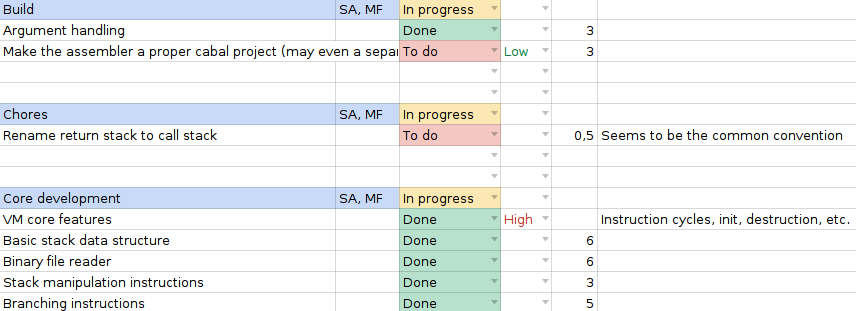
\includegraphics[width=.9\textwidth]{./images/backlog}

  \caption{Excerpt from the initial backlog}
  \label{fig:project-mgm:backlog}
\end{figure}

\subsection{Technical Management}

When working in a team with multiple developers it is of paramount importance to
efficiently manage the codebase. When multiple people are writing code in the
same source tree it is virtually impossible to manually maintain and apply
changes from each other. Further it is an invaluable tool to be able to revert
changes and work on different branches of the system in a unified manner, which
is true for both a single person project and for teams of a dozen developers for
the same codebase.

Specifically designed for this purpose are Source Code Management (SCM)
tools. Without going into excessive details, there two general forms of SCMs
which differ fundamentally in the way files can be edited concurrently. The
\textit{centralized} model (Microsoft TFS, Subversion) uses a central code
repository from which everyone edits files and is the single source of
truth. With \textit{decentralized} SCMs every developer has her own repository
and can merge changes from servers or other developers directly. There is no
single source of truth in this model, but a mainline tree is almost always
maintained.

The SCMs handle merging of files which have been edited by multiple people, and
are very good at doing this automatically. They can obviously not resolve merges
where the same lines of code have been changed differently, and so the developer
has to resolve the conflicting parts manually.

We have used the git\footnote{Git Source Control Management:
  \url{http://git-scm.com}} SCM tool which is fully decentralized which we find
to be the most convenient model.

\subsection{Evalutation of the Management Process}

We followed the phase structure described in
Section~\ref{sec:project-mgmt:phases} starting with the inception phase and got
the vision and overarching plan of the project laid out. During the elaboration
we began to keep a backlog as concrete work started, both in terms design and
programming tasks. Programming tasks were fairly easy to describe and can be
well isolated, though many of them were inevitably interdependent and had to be
carried out in a specific order. However we quickly found that design tasks are
very difficult to describe in detail and even more so to estimate. This is both
due to the fact that describing a design task is essentially part of solving it,
and that the time it takes to figure out a design decision is highly
unpredictable. It becomes even more complicated when design flaws are discovered
and development plans must change. For several purposes it did not prove
beneficial to use the backlog strictly, but instead generated unnecessary
overhead, why we began to use it more ad-hoc.

As for planning of sprints we used the weekly meetings with our advisor as
milestones where we summarized the work that had been done and the plan for the
next week. That way we could get continuous feedback on the plan which was a
great help in taking the project in the right direction.

In the final weeks of the project we shifted from the spreadsheet backlog to
somewhat extensive to-do lists using a tool for the Emacs editor known as
org-mode\footnote{Org-mode for Emacs: \url{http://orgmode.org}} (for
organization mode). It enables nested lists of items with descriptions and
current status as well as tagging mechanisms. The main down-side of org-mode is
that it cannot be shared between the both of us, but because we were always
working at the same location it was not a significant issue.

We have certainly learned that good planning is vital for a successful project
process, and that it pays off to thoroughly weigh and examine design choices
before starting an implementation. It is a fine balance between management and
production and there will never be a single method that works for all types of
projects. We consider the essence of the agile methodology useful, but the
process must be tailored to each individual project. The concrete methods used
must depend of the type of software that is being developed, what the relation
to the end-user is, how it is going to be deployed (continuous delivery,
milestone based or a single one-time delivery), the size of the team and so
on. There is also a substantial difference between working for paying customers
and doing an academic project, the latter of which tends to change more than the
former as the project progresses.

%%% Local Variables:
%%% mode: latex
%%% TeX-master: "../report"
%%% End:


\clearpage
\section{Conclusions}
\label{sec:conclusions}
The problem that \thename{} attempts to solve is a complex matter that spans a
wide range of areas in the field of computer science. As a result our work on
the implementation has involved a great deal of different types of work, varying
from instruction set design and executable file formats, to efficient hash maps
and C code architecture.

Along the way we have gained a thorough knowledge of the internals of abstract
machines and code interpretation in general. We have come to realize that it is
no simple task to build a machine that is capable of expressing most of the
modern programming language paradigms in a unified manner. In addition we have
discovered the immense value and assurance that extensive tests provides.

Implementing a machine like \thename{} has been an interesting experience in
terms of working on a non-trivial and relatively low-level software project
using an agile workflow that allowed us to cope with regular changes.

We have achieved a result that can serve as evidence that the vision of
\thename{} is indeed possible. Our benchmarkings revealed that the run-time
performance in most cases is sub-optimal for practical uses, but does not fall
far behind the Java Virtual Machine is isolated cases. The general maturity of
the machine is not on par with the existing industrial strength systems, but it
does do a good job of implementing the fundamental semantics in a different way
that could be the cornerstone for future work.

%%% Local Variables:
%%% mode: latex
%%% TeX-master: "../report"
%%% End:


\newpage
% \nocite{*}
\printbibliography[heading=bibintoc]

\appendix
\section{Appendices}
\label{sec:appendices}
\subsection{Running \thename{}}
\label{sec:appendix:make}

Building \thename{} is a simple matter of using the GNU Make build tool. In the
root folder containing the file \code{Makefile}, simply run the command
\code{make} to build and run the machine with the hardcoded test program.

Tests are likewise run via make using the command \code{make test}. Valgrind
analysis and gprof profiling is performed with \code{make analyze} and
\code{make gprof}, respectively.

\subsection{\thename{} Specification}
\label{sec:appendix:spec}
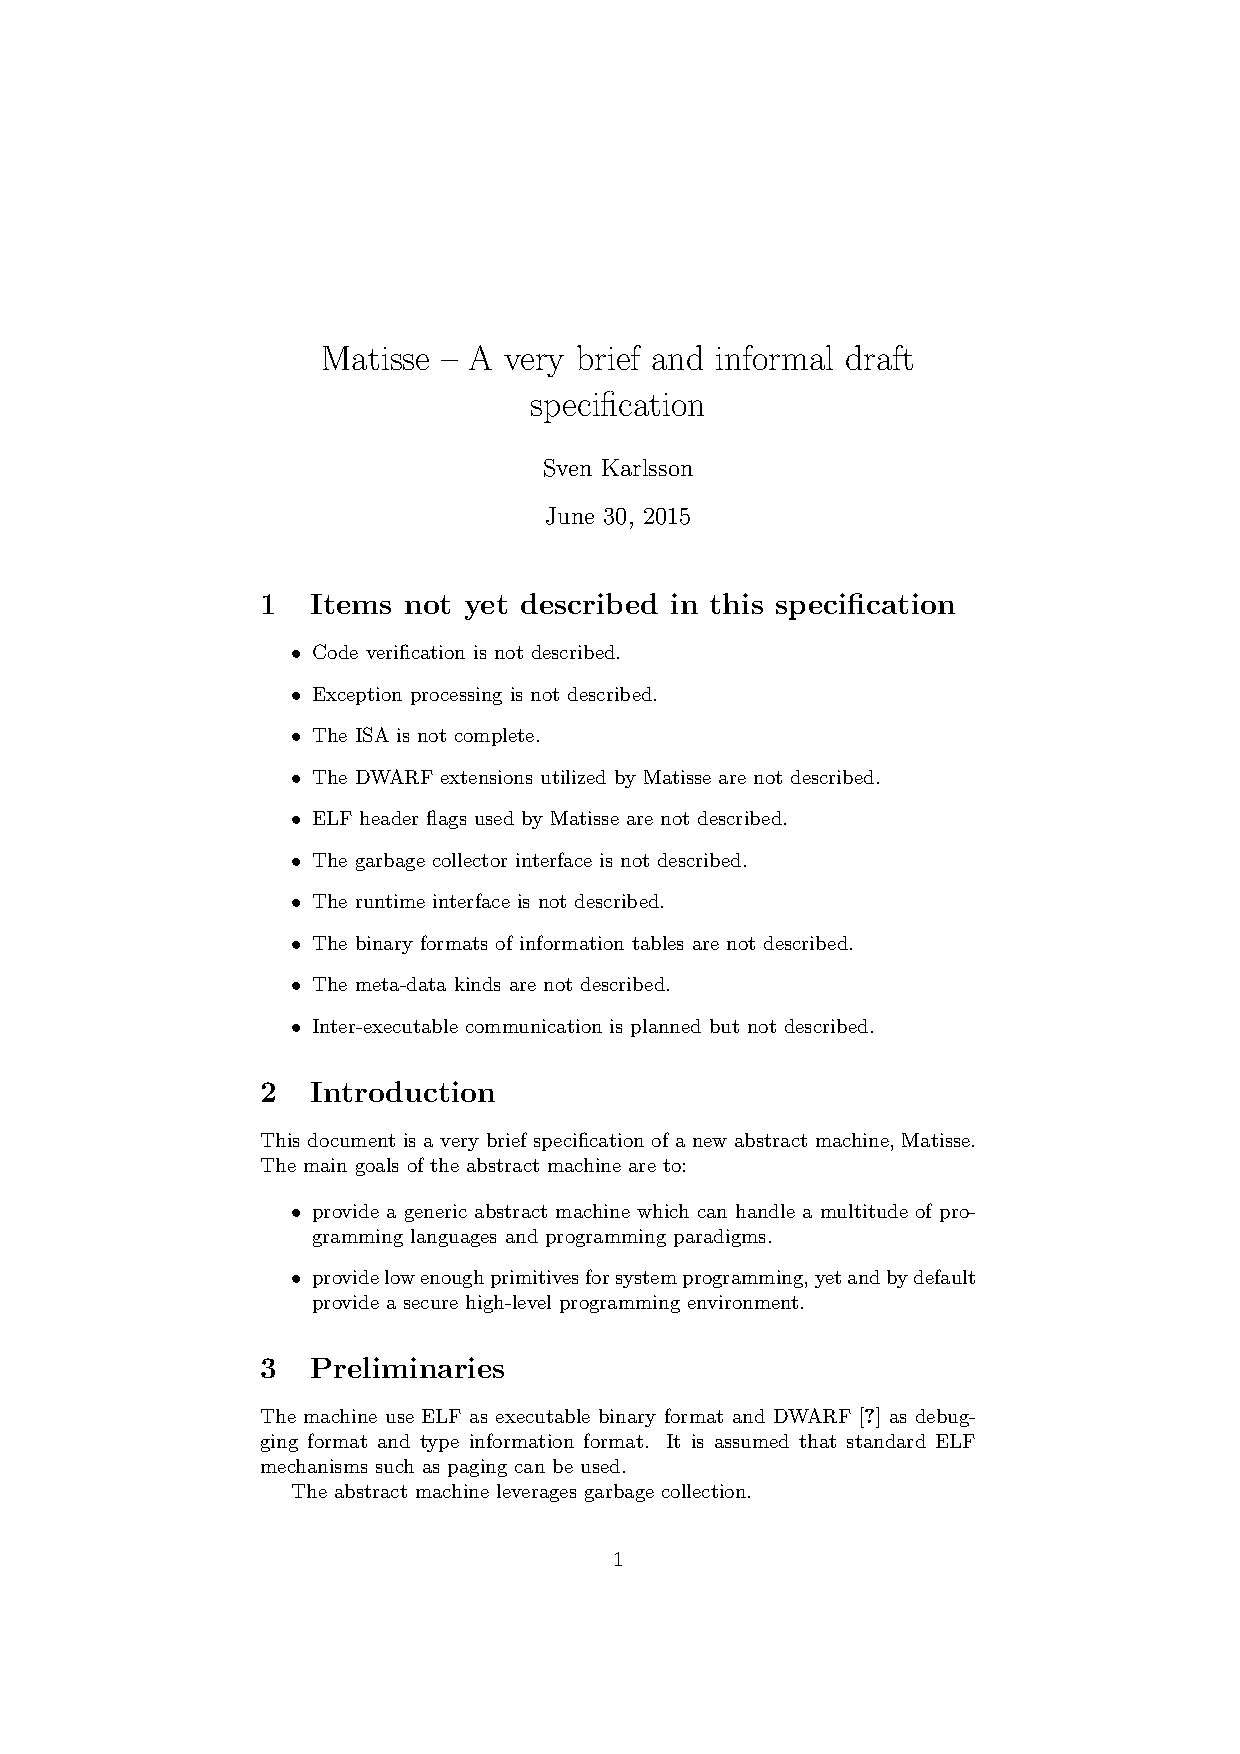
\includepdf[pages=-]{lib/spec.pdf}

\subsection{Project Inception Phase Artifact}
\label{appendix:inception-artifact}

\includepdf[pages=-]{lib/Inception.pdf}

\subsection{Benchmark Runner}
\label{appendix:benchmark}
\begin{lstlisting}[language=bash]
#!/usr/bin/bash
# benchmark runner
# based off:
# https://gist.github.com/peterjmit/3864743

repeat=1
step=1
range_from=0
range_to=30
output_file="benchmark.csv"
command=""

run_tests() {
    echo "benchmarking: ${command} ${range_from}..${range_to} (step ${step})"

    # truncate output file
    if [ -f ${output_file} ]
    then
        > ${output_file}
    fi

    # print column names
    echo "round,n,time,user,kernel" >> ${output_file}

    # repeat
    for (( j = 0; j < ${repeat}; j++ ))
    do
        # for each in range
        for (( i = ${range_from}; i < ${range_to}; i += ${step} ))
        do
            # percentage completion
            p=$(( ($i + 1) * 100 / $range_to ))
            # indicator of progress
            l=$(seq -s "#" $(($p / 2)) | sed 's/[0-9]//g')

            # time command
            /usr/local/bin/time -f "${j},${i},%e,%U,%S" -o ${output_file} -a ${command} ${i} > /dev/null

            # clear the HDD cache (i hope?)
            sync && echo 3 > /proc/sys/vm/drop_caches

            printf "%s/%s: %-48s %3s%%\r" "$(($j + 1))" "$repeat" "$l" "$p"
        done
    done

    echo -ne '\n'
}

# Option parsing
while getopts s:f:t:n:c:o: OPT
do
    case "$OPT" in
        s)
            step=$OPTARG
            ;;
        f)
            range_from=$OPTARG
            ;;
        t)
            range_to=$OPTARG
            ;;
        n)
            repeat=$OPTARG
            ;;
        o)
            output_file=$OPTARG
            ;;
        c)
            command=$OPTARG
            ;;
        \?)
            echo 'error: failed to parse args'
            exit 1
            ;;
    esac
done

shift `expr $OPTIND - 1`

if [[ $command == "" ]]
then
    echo 'error: no command to run'
    exit 1
fi

run_tests
\end{lstlisting}

%%% Local Variables:
%%% mode: latex
%%% TeX-master: "../report"
%%% End:

% Instruction set listing
% Complete backlog

\end{document}

%%% Local Variables:
%%% mode: latex
%%% TeX-master: t
%%% End:
